% !TeX TS-program = xelatex
% !TeX root = kristallographie_skript.tex
% !TeX spellcheck = de_DE
\documentclass[fontsize=11pt,fleqn,a4paper]{scrartcl}

%%% Language preamble for german

% Language itself
\usepackage[ngerman]{babel}
% Font encoding to represent umlauts correct in PDFs documents instead of combining them from other
% characters like "u instead of ü
\usepackage[T1]{fontenc}
% Encoding of the source code.
\usepackage[utf8]{inputenc}


% Language specific strings
%   Names of theorem environments

%\makeatletter
\addto\captionsngerman{
	% \see command from makeidx
%	\@ifpackageloaded{makeidx}{
%		\renewcommand{\seename}{siehe}
%	}{}
	\renewcommand{\captionstringtheorem}{Satz}
	\renewcommand{\captionstringlemma}{Lemma}
	\renewcommand{\captionstringcorollary}{Korollar}
	\renewcommand{\captionstringlemmadef}{Lemma und Definition}
	\renewcommand{\captionstringtheoremdef}{Satz und Definition}
	\renewcommand{\captionstringdefinition}{Definition}
	\renewcommand{\captionstringproposition}{Proposition}
	\renewcommand{\captionstringexample}{Beispiel}
	\renewcommand{\captionstringconjecture}{Vermutung}
	\renewcommand{\captionstringconvention}{Vereinbaring}
	\renewcommand{\captionstringremark}{Bemerkung}
}
%\@ifpackageloaded{biblatex}{
%\DefineBibliographyStrings{german}{
%	bibliography = {Bibliographie},
%	references = {Referenzen}
%}
%}{}
%\makeatother
%%% General math packages

% AMS
\usepackage{amsmath,  
            amssymb,  % Symbols
            amsthm,   % provides theorem environments
            amsfonts  % fonts like \mathbb and \mathfrak
            }

% useful things for math typesetting like \smash, \psmallmatrix, ...
\usepackage{mathtools}

% For \Set and \set. Automatic resizing of the curly braces and the middle vertical line
\usepackage{braket}   

% For even more extensible arrows
\usepackage{extpfeil} 

% Blockmatrices
%\usepackage{multirow}

% and brakets around matrix rows
%\usepackage{bigdelim}


%%% Own symbols and operators
\newcommand{\IN}{\mathbb{N}}
\newcommand{\IZ}{\mathbb{Z}}
\newcommand{\IQ}{\mathbb{Q}}
\newcommand{\IR}{\mathbb{R}}
\newcommand{\IC}{\mathbb{C}}
\newcommand{\IK}{\mathbb{K}}

\DeclarePairedDelimiter{\abs}{\lvert}{\rvert}
\DeclarePairedDelimiter{\norm}{\lVert}{\rVert}
\DeclarePairedDelimiter{\ceil}{\lceil}{\rceil}
\DeclarePairedDelimiter{\floor}{\lfloor}{\rfloor}

\newcommand{\isomorphic}{\cong}
\newcommand{\homotopic}[1][]{\overset{#1}{\simeq}}

\renewcommand{\Im}{\operatorname{\mathfrak{Im}}}
\renewcommand{\Re}{\operatorname{\mathfrak{Re}}}

\DeclareMathOperator{\id}{id}
\DeclareMathOperator{\Hom}{Hom}
\DeclareMathOperator{\End}{End}
\DeclareMathOperator{\Aut}{Aut}
\DeclareMathOperator{\Sym}{Sym}
\DeclareMathOperator{\Isom}{Isom}

\DeclareMathOperator{\tr}{tr}
\DeclareMathOperator{\sgn}{sgn}
\DeclareMathOperator{\ord}{ord}

\DeclareMathOperator{\im}{im}

%%% Theorem environments

% Define name strings
\newcommand{\captionstringtheorem}{Theorem}
\newcommand{\captionstringlemma}{Lemma}
\newcommand{\captionstringcorollary}{Corollary}
\newcommand{\captionstringlemmadef}{Lemma and definition}
\newcommand{\captionstringtheoremdef}{Theorem and definition}
\newcommand{\captionstringdefinition}{Definition}
\newcommand{\captionstringproposition}{Proposition}
\newcommand{\captionstringexample}{Example}
\newcommand{\captionstringconjecture}{Conjecture}
\newcommand{\captionstringconvention}{Convention}
\newcommand{\captionstringremark}{Remark}


% Definition of two similar styles
\newtheoremstyle{dotless} % Name
			{\bigskipamount}    % Space above
			{\bigskipamount}    % Space below
			{\nopagebreak}      % Body font, also suppress pagebreak between "Theorem 3.14:" and text
			{}                  % Indent amount
			{\bfseries}         % Theorem head font
			{:}                 % Punctuation after theorem head
			{\newline}          % Space after theorem head
			{}                  % Theorem head spec (can be left empty, meaning 'normal')
\newtheoremstyle{dotless2} % Name
			{\bigskipamount}    % Space above
			{0.0em}             % Space below
			{}                  % Body font
			{}                  % Indent amount
			{\bfseries}         % Theorem head font
			{:}                 % Punctuation after theorem head
			{0.5em}             % Space after theorem head
			{}                  % Theorem head spec (can be left empty, meaning 'normal')
% "3.14 Theorem" instead of "Theorem 3.14"
\swapnumbers

\newcounter{theoremnumber}
\numberwithin{theoremnumber}{section}

\theoremstyle{dotless}
\newtheorem{theorem}[theoremnumber]{\captionstringtheorem}
\newtheorem{theoremdef}[theoremnumber]{\captionstringtheoremdef}
\newtheorem{lemma}[theoremnumber]{\captionstringlemma}
\newtheorem{lemmadef}[theoremnumber]{\captionstringlemmadef}
\newtheorem{corollary}[theoremnumber]{\captionstringcorollary}
\newtheorem{proposition}[theoremnumber]{\captionstringproposition}
\newtheorem{definition}[theoremnumber]{\captionstringdefinition}
\newtheorem{example}[theoremnumber]{\captionstringexample}
\newtheorem{conjecture}[theoremnumber]{\captionstringconjecture}

\newtheorem*{convention}{\captionstringconvention}

\theoremstyle{dotless2}
\newtheorem{remark}[theoremnumber]{}


%%% Math style file

% Sets the strictness of handling page breaks inside align-Umgebungen
% Level [1] breaks will be avoided if possible,
% Levels [2], [3], [4] are increasingly relaxed.
\allowdisplaybreaks[1]


%%% Everything tikz

\usepackage{tikz}
\usetikzlibrary{arrows}
\usetikzlibrary{cd}

% Predefine styles
\tikzset
{
	desc/.style=
	{
		fill=white,inner sep=2pt,font=\scriptsize
	}
}


%%%% Styles for algorithms

\usepackage{listings}
\lstset{%
	basicstyle = \ttfamily\small,
	tabsize = 3
}
% Use theorem environment for algorithm descriptions
\newtheorem{algorithm}{Algorithmus}
% Change numbering of algorithms to include chapter
\renewcommand{\thealgorithm}{\Alph{chapter}.\Roman{algorithm}}
%%%% Tables and figures
\numberwithin{table}{section}
\numberwithin{figure}{section}



%%% Text styles

% For the interrobang
\usepackage{textcomp}

% Additional underlining options, especially dotted underlining, line breaks in underlined text etc.
\usepackage[normalem]{ulem} % option not to change look of \emph{}
\newcommand*{\udot}{\dotuline}


% Skip lengths
\setlength{\parindent}{0em}
\setlength{\parskip}{0em}


% Pimp enumerate and itemize environments. More counter options and resuming numbering
\usepackage{enumitem}

% Style of enumerations and itemizations
\renewcommand{\labelenumi}{\alph{enumi}.)}  % Counter enumi wird immer als a.) b.) c.) dargestellt.
\renewcommand{\labelenumii}{\roman{enumii}.)}  % Counter enumii wird immer als i.) ii.) iii.) dargestellt.


\usepackage{csquotes}

\usepackage{multicol}
%%%% Bibliography with BibTeX only

\usepackage[numbers]{natbib}
\bibliographystyle{plain}


%%%% Bibliography with biblatex + bibtex

\usepackage[
	style=alphabetic,
	sorting=nty,
	url=false,
	natbib=true,
	backend=biber,  % Biber backend
	defernumbers=true
]{biblatex}
% The .bib-file(s) for this document
\addbibresource{wgraph.bib}


%%%% Bibliography with biblatex + bibtex

\usepackage[
	style=alphabetic,
	sorting=nty,
	url=false,
	natbib=true,
	backend=biber,  % Biber backend
	defernumbers=true
]{biblatex}
% The .bib-file(s) for this document
\addbibresource{wgraph.bib}



% !! Hyperref before imakeidx !!
%%% PDF stuff
%%%
%%% Include hyperref before imakeidx !!

\usepackage[
	pdfpagelabels=true,
	plainpages=false
	]{hyperref}
	
\hypersetup{
colorlinks=true,
linkcolor=red,
urlcolor=blue,
citecolor=blue,
linktocpage=true, % Page numbers will be the links in t.o.c instead of the headings themselves
pdfpagelayout={OneColumn},
pdfstartview= % empty to cause the viewer to use its preferred behaviour instead of dictating a behaviour at opening of the document
}

\makeatletter
{\hypersetup{
pdfinfo=
	{  
		Title={\@title},
		Author={\@author},
		Keywords={Space groups, point groups, bravais lattices},
		Subject={Crystallography}
	}
}}
\makeatother
%\input{_preamble/indicies.tex}

\title{Kristallographie}
\author{Johannes Hahn \and Andrea Hanke}

\begin{document}

\maketitle

\section{Geometrie}
% !TeX spellcheck = de_DE
% !TeX root = kristallographie_skript.tex
\begin{definition}
Eine \udot{starre Bewegung} oder \udot{Isometrie} ist eine Abbildung $\phi:\IR^n\to\IR^n$, die abstandserhaltend ist, d.h.
\[\forall x,y\in\IR^n: \norm{\phi(x)-\phi(y)} = \norm{x-y}\]
\end{definition}

\begin{example}
\begin{enumerate}
\item Translationen: $\tau_v(x) := x+v$.
\item Drehungen im $\IR^3$: Bis auf Koordinatenwahl die Abbildungen der Form
\[\begin{pmatrix}x\\y\\z\end{pmatrix}\mapsto\begin{pmatrix}
\cos(\alpha)x + (-\sin(\alpha)) y \\
\sin(\alpha)x + \cos(\alpha)y \\
z
\end{pmatrix}\]
$\alpha$ wird dabei als Drehwinkel bezeichnet. Die Drehachse erkennt man daran, dass es eine Gerade $A\subseteq\IR^3$ ist, die $D(A)=A$ erfüllt. In obiger Beschreibung ist das Koordinatensystem so gewählt worden, dass die Drehachse genau die Gerade $\Set{\begin{psmallmatrix}0\\0\\z\end{psmallmatrix} | z\in\IR}$ ist.
\item Inversionen = Punktspiegelungen
\item Spiegelungen an einer Geraden (in $\IR^2$) bzw. an einer Ebene (in $\IR^3$) bzw. allgemein an einer Hyperebene ($(n-1)$-dimensionale Unterräume von $\IR^n$).
\item Wenn $f,g$ Isometrien sind, dann auch $f\circ g$, z.B.
\begin{enumerate}
\item Gleitspiegelungen: Im eine Spiegelung an einer Geraden (in $\IR^2$), einer Ebene (im $\IR^3$) bzw. allgemeiner einer Hyperebene gefolgt von einer Translation in Richtung eines Vektors parallel zu dieser Geraden / Ebene / Hyperebene.
\item Drehinversionen: Eine Drehung $g$ gefolgt von einer Inversion $f$ in einem Punkt auf der Drehachse von $g$.
\item Schraubungen: Eine Drehung $g$ gefolgt von einer Translation $f$ entlang der Drehachse.
\end{enumerate}
\item Die Identität $\id: x\mapsto x$. Das ist gleichzeitig die Translation um die Distanz $0$ (in jede Richtung) und die Drehung um den Winkel $0$ (mit jeder Drehachse).
\end{enumerate}
\end{example}

\begin{table}[htp]
	\caption{Symbolnotationen für Bewegungen ohne Translationsanteil}
	\begin{tabular}{cC{4cm}C{5cm}c}
		\toprule
		Symbol    & Hermann-Maguin-Symbol       & Symmetrien                                  & Gruppenordnung \\
		\midrule
		\sym{0}   & $\overline{1}$                             & Inversion                                   & 1              \\
		\sym{2}   & $2$                                        & 2-zählige Drehung                           & 1              \\
		\sym{3}   & $3$                                        & 3-zählige Drehung                           & 3              \\
		\sym{4}   & $4$                                        & 4-zählige Drehung                           & 4              \\
		\sym{6}   & $6$                                        & 6-zählige Drehung                           & 6              \\
		\sym{20} & $m \hspace{0.5cm}(=\overline{2})$           & Ebenenspiegelung                            & 2              \\
		\sym{30}  & $\overline{3}$ \enquote{drei quer}         & 3-zählige Drehinversion                     & 6              \\
		\sym{84}  & $\overline{4}$ \enquote{vier quer}         & 4-zählige Drehinversion                     & 4              \\
		\sym{36}  & $\overline{6}$ \enquote{sechs quer}        & 6-zählige Drehinversion                     & 6              \\
		\sym{102} & $\frac{2}{m}$ \enquote{zwei über m}        & Spiegelung \& 2-zählige Drehung um Spiegelebenennormale & 4              \\
		\sym{103} & $\frac{3}{m} = \overline{6}$ \enquote{drei über m} & Spiegelung \& 3-zählige Drehung um Spiegelebenennormale & 6 \\
		\bottomrule
\label{table:symbole_punkt}
	\end{tabular}

	\bigskip
	
	\caption{Symbolnotationen für Bewegungen mit Translationsanteil}
	\begin{tabular}{C{1.5cm}C{3cm}C{5cm}C{3cm}c}
		\toprule
		Symbol                                                       & Hermann-Maguin-Symbol       & Symmetrien mit Translation um $t$                                                                                                                                                                       & Ordnung der induzierten Punktgruppe & \\
		\midrule
		\sym{21}                                                     & $2_1$                                      & 2-zählige Schraubung, $t=\frac{1}{2}$                                                                                                                                                                       & 2                      &  \\
		\sym{31} \ \  \sym{32}                                       & $3_1$ \ \  $3_2$                           & 3-zählige Schraubung, $t=\frac{1}{3}, t=\frac{2}{3}$                                                                                                                                                       & 3                       & \\
		\sym{41}\ \  \sym{42} \ \ \sym{43}                           & $4_1$ \ \ $4_2$ \ \newline $4_3$                  & 4-zählige Schraubung, $t=\frac{1}{4}, t=\frac{2}{4}, t=\frac{3}{4}$                                                                                                                                        & 4                        & \\
		\sym{61} \ \ \sym{62} \ \ \sym{63} \ \ \sym{64} \ \ \sym{65} & $6_1 \ \ 6_2$ \ \newline $6_3$ \ \ $6_4$ \ \newline $6_5$ & 6-zählige Schraubung, $t=\frac{1}{6}, t=\frac{2}{6}, t=\frac{3}{6},$\newline$ t=\frac{4}{6}, t=\frac{5}{6}$                                                                                                          & 6                       & \\
		\sym{9}                                                      & $a, b, c, n, d$                            &  Gleitspiegelung, $t=\frac{1}{2}\vc{a}, t=\frac{1}{2}\vc{b}, t=\frac{1}{2}\vc{c}, t=\frac{1}{2}(\vc{\tau_1}+\vc{\tau_2}), t=\frac{1}{4}(\vc{\tau_1} +\vc{\tau_2}) $ & 2, 4 & \\                  
		\bottomrule
\label{table:symbole_raum}
	\end{tabular}
\end{table}

\begin{definition}
Angenommen, wir haben einen Nullpunkt gewählt. Eine Isometrie, die den Nullpunkt fixiert, wird \udot{orthogonale} Abbildung genannt.
\end{definition}

\begin{theorem}
Es sei $f:\IR^n\to\IR^n$ eine Bewegung. Dann gilt:
\begin{enumerate}
\item $f$ ist \udot{affin}, d.h.
\[\forall p_0,p_1\in\IR^n, \lambda\in\IR: f(\lambda p_1 + (1-\lambda)p_0) = \lambda f(p_1)+(1-\lambda)f(p_0)\]
\item Haben wir einen Nullpunkt gewählt und ist $f$ orthogonal, dann ist $f$ sogar \udot{linear}, d.h.
\begin{enumerate}
\item $\forall v_1,v_2\in\IR^n: f(v_1+v_2)=f(v_1)+f(v_2)$
\item $\forall v\in\IR^n, \lambda\in\IR: f(\lambda v)=\lambda f(v)$.
\end{enumerate}
\item $f$ erhält das Skalarprodukt von Vektoren und Winkel zwischen Vektoren.
\end{enumerate}
\end{theorem}
\begin{proof}
a. Sei zunächst $0\leq \lambda\leq 1$. Der Punkt $\lambda p_1+(1-\lambda)p_0 = p_0+\lambda(p_1-p_0) = p_1-(1-\lambda)(p_1-p_0)$ ist genau derjenige Punkt, der genau Abstand $\lambda\norm{p_1-p_0}$ von $p_0$ und $(1-\lambda)\norm{p_1-p_0}$ von $p_1$ hat und es gibt nur einen solchen Punkt. Daher ist $f(\lambda p_1+(1-\lambda)p_0)$ genau derjenige Punkt, der den Abstand $\lambda\norm{p_1-p_0}=\lambda\norm{f(p_1)-f(p_0)}$ von $f(p_0)$ und den Abstand $(1-\lambda)\norm{p_1-p_0} = (1-\lambda)\norm{f(p_1)-f(p_0)}$ von $f(p_1)$ hat. Weil es nur einen solchen Punkt gibt, muss $f(\lambda p_1+(1-\lambda)p_0) = \lambda f(p_0)+(1-\lambda)f(p_1)$ sein.

Im allgemeinen Fall liegen die drei Punkte $p_0$, $p_1$ und $p_\lambda:=\lambda p_1+(1-\lambda)p_0$ ja auf einer gemeinsamen Geraden. Es gibt also immer einen, der zwischen den anderen zweien positioniert ist. Wenn das z.B. $p_0$ ist, dann gibt es eine Gleichung der Form $p_0 = \alpha p_\lambda + (1-\alpha)p_1$ mit $\alpha\in [0,1]$ (Übung: Man berechne $\alpha$ aus $\lambda$ und umgekehrt). Wenn $p_1$ zwischen $p_0$ und $p_\lambda$ liegt, gibt es analog eine Gleichung der Form $p_1=\beta p_\lambda + (1-\beta)p_1$ mit $\beta\in[0,1]$. In beiden Fällen folgt aus dem schon bewiesenen auch die gleiche Gleichung für $f(p_0)$, $f(p_1)$ und $f(p_\lambda)$.

\medbreak
b. Wenn $f(0)=0$ ist, dann können wir $p_0=0$ und $p_1=v$ in a. einsetzen und erhalten direkt, dass $f(\lambda v)=\lambda f(v)$ gilt.

Daraus folgern wir nun:
\[f(v_1+v_2) = 2f(\tfrac{1}{2}(v_1+v_2)) = 2f(\tfrac{1}{2}v_1 + \tfrac{1}{2}v_2) \overset{a.}{=} 2(\tfrac{1}{2}f(v_1)+\tfrac{1}{2}f(v_2))=f(v_1)+f(v_2)\]

\medbreak
c. folgt aus $\tfrac{1}{2}(\norm{v_1+v_2}^2-\norm{v_1}^2-\norm{v_2}^2)=\braket{v_1,v_2}$, $\norm{v}=\norm{f(v)}$ und b.

Winkelerhaltung folgt dann aus $\cos(\sphericalangle(v_1,v_2)) = \frac{\braket{v_1,v_2}}{\norm{v_1}\cdot\norm{v_2}}$.
\end{proof}

\begin{remark}
Aus der Linearität und der Tatsache, dass wir nur Räume endlicher Dimension betrachten, kann man folgern, dass jede Isometrie bijektiv ist, also eine Umkehrabbildung besitzt. Die Umkehrabbildung muss dann selbst wieder eine Isometrie sein, denn:
\[\norm{p_1-p_2} = \norm{f(f^{-1}(p_1))-f(f^{-1}(p_2))} = \norm{f^{-1}(p_1)-f^{-1}(p_2)}\]
\end{remark}

\subsection{Klassifikation der Bewegungen}

\begin{lemma}[Reduktion von beliebigen auf orthogonale Bewegungen]
Haben wir einen Nullpunkt gewählt, dann ist ein beliebiges $f\in\Isom(\IR^n)$ eine orthogonale Abbildung gefolgt von einer Translation (mglw. um den Abstand $0$).
\end{lemma}
\begin{proof}
Ist $f(0)=:v$, dann betrachten wir die Translation $\tau_v$. Dann ist nämlich $(\tau_v^{-1}\circ f)(0) = 0$, also ist $f=\tau_v\circ(\tau_v^{-1}\circ f)$ eine Komposition aus der orthogonalen Abbildung $\tau_v^{-1}\circ f$ gefolgt von der Translation $\tau_v$.
\end{proof}

\begin{theorem}[Klassifikation von Bewegungen in kleinen Dimensionen]
Alle orthogonalen Abbildungen des
\begin{enumerate}
\item $\IR^1$ sind die Identität oder Spiegelung im Nullpunkt.
\item $\IR^2$ sind Drehungen (ggf. um den Winkel $0$) um den Nullpunkt oder Spiegelungen an Geraden durch den Nullpunkt.
\item $\IR^3$ sind Drehungen oder Drehinversionen (ggf. um den Drehwinkel $0$) um eine Achse durch den Nullpunkt oder Ebenenspiegelungen an Ebenen durch den Nullpunkt.
\end{enumerate}

Allgemeiner: Alle Bewegungen des
\begin{enumerate}
\item $\IR^1$ sind Translationen oder Spiegelungen.
\item $\IR^2$ sind Drehungen (ggf. um den Drehwinkel $0$) oder Geradenspiegelungen gefolgt von einer Translation (ggf. um den Abstand $0$).
\item $\IR^3$ sind Drehungen oder Drehinversionen (ggf. um den Drehwinkel $0$) oder Ebenenspiegelungen gefolgt von einer Translation (ggf. um den Abstand $0$).
\end{enumerate}
\end{theorem}

\subsection{Stereographische Projektion}
Mittels der \udot{stereographischen Projektion} werden alle Punkte auf der Kugeloberfläche von $S^2$ bis auf dem Südpol als Punkte auf einer Ebene dargestellt. Wir nutzen sie, um Orientierungen von Vektoren im dreidimensionalen Raum zueinander im zweidimensionalen Raum darzustellen. Diese Vektoren können verschiedenes symbolisieren, bei uns meist die Orientierung von Drehachsen und Flächennormalen von konvexen Körpern.
\begin{figure}%{0.5\linewidth}
\centering
\begin{subfigure}{0.4\textwidth}
	\centering
	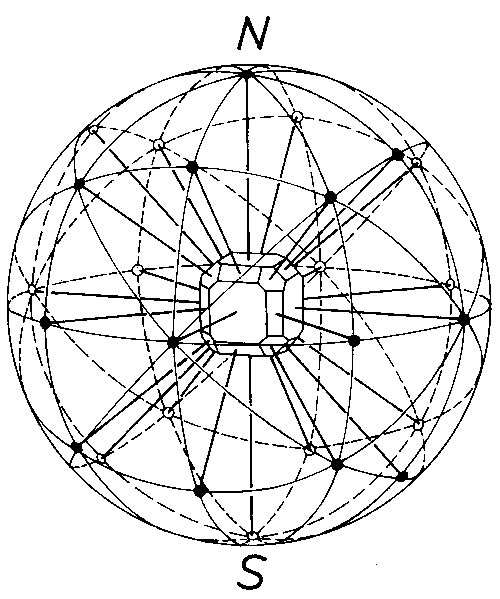
\includegraphics[width=0.8\linewidth]{./pictures/stpr1.jpg}
	\caption{Schnittpunkte der Flächennormalen auf $S^2$}
\end{subfigure}%
\begin{subfigure}{0.4\textwidth}
	\centering
	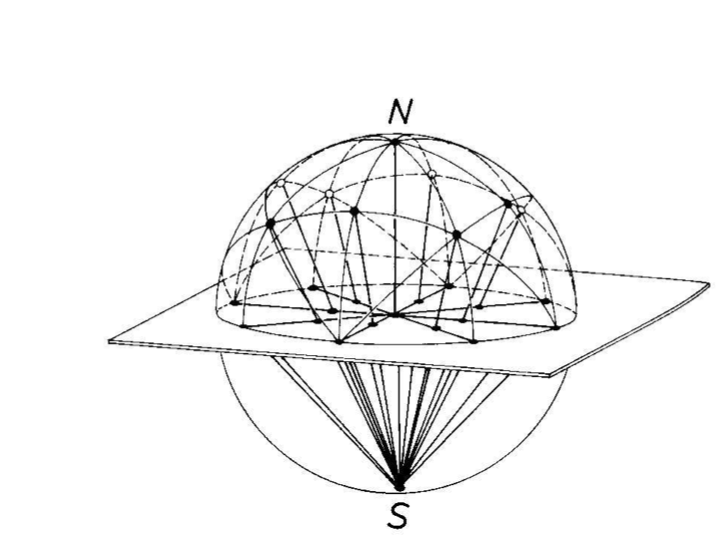
\includegraphics[width=1.2\linewidth]{./pictures/stpr2.jpg}
	\caption{Projektion auf die Äquatorebene}
\end{subfigure}
\caption{Stereographische Projektion eines konvexen Körpers}
\end{figure}

\begin{figure}
	\centering
	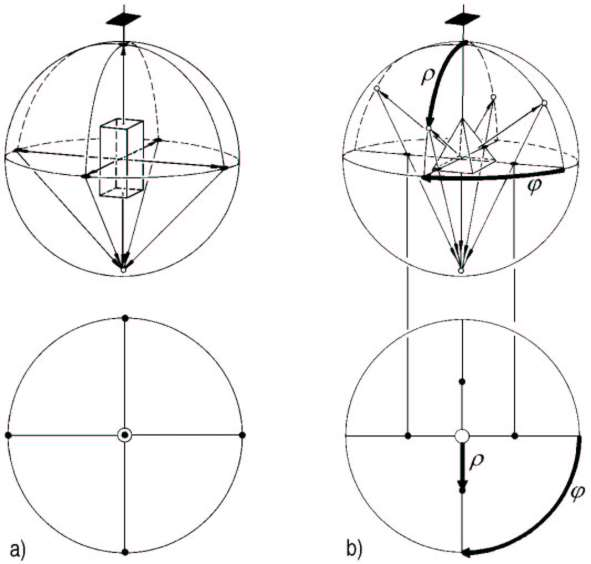
\includegraphics[width=0.8\linewidth]{./pictures/stpr3.jpg}
	\caption{Stereographische Projektion verschiedener Körper}
\end{figure}

\begin{figure}
	\centering
\begin{subfigure}{1\textwidth}
	\centering
	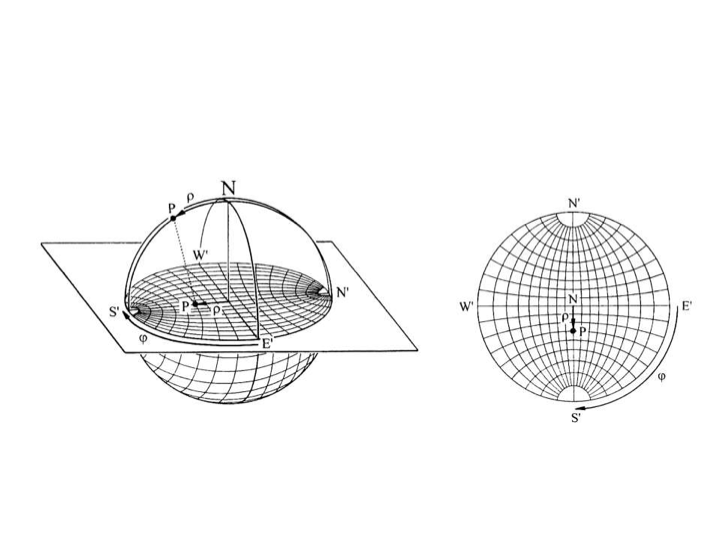
\includegraphics[width=1.1\linewidth]{./pictures/stpr4.jpg}
	\caption{Lage der Winkel $\phi$ und $\rho$}
\end{subfigure}
\begin{subfigure}{0.9\textwidth}
	\centering
	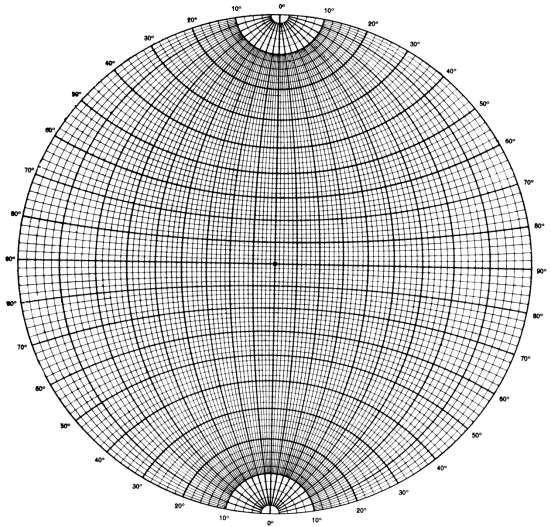
\includegraphics[width=0.8\linewidth]{./pictures/stpr5.jpg}
	\caption{Das Wulffsche Netz}
\end{subfigure}
	\caption{Orientierung ablesen mit dem Wulffschen Netz}
\end{figure}
 Dazu nutzen wir eine Kugel mit Oberfläche $S^2$, Mittelpunkt $m$, Nordpol $N$, Südpol $S$ und Äquatorebene $A$. Die Vektoren, die wir darstellen wollen, verlängern wir zu von $m$ ausgehenden Halbgeraden, die $S^2$ in einem Schnittpunkt $p$ schneiden. Jeder dieser Schnittpunkte $p$ wird mit einer Geraden mit dem Südpol der Kugel verbunden. Der Schnittpunkt $a$ einer solchen Geraden mit der Äquatorebene ist die Projektion des Vektors.
 Diese stereographische Projektion ist winkelerhaltend (aber nicht abstandserhaltend) und eignet sich daher, Orientierungen  (aber keine Tranlationen) in 3D auf einem (unendlich großen) Stück Papier darzustellen. Man beachte, dass bei dieser Konstruktion alle Punkte auf der Nordhalbkugel innerhalb des Äquatorkreises projiziert werden, der Äquator auf sich selbst abgebildet wird und alle Punkte der Südhalbkugel außerhalb des Äquators landen. 

Eine in der Kristallographie oft verwendete Variation der stereographischen Projektion ist die folgende: Alle Punkte der Nordhalbkugel werden mit dem Südpol verbunden und die Schnittpunkte werden mit einem Kreuz gekennzeichnet. Alle Punkte der Südhalbkugel werden hingegen mit dem Nordpol verbunden und die Schnittpunkte werden mit einem Kreis gekennzeichnet. Dadurch braucht es nur noch ein endlich großes Stück Papier (nämlich genau die Fläche, die durch den Äquator eingeschlossen wird).
Oft wird diese (kristallographische) Stereographische Projektion benutzt, um 3-dimensionale konvexe Körper darzustellen. Dazu werden die Normalenvektoren aller Flächen vom Körper wie oben beschrieben projiziert. Man kann sich auch vorstellen, dass der Mittelpunkt des konvexen Körpers auf dem Mittelpunkt $m$ der Kugel sitzt und dann die Flächennormalen verlängern, bis sie $S^2$ durchstoßen. Aber Achtung: Der Ursprung der projizierten Flächennormalen des konvexen Körpers ist nicht frei wählbar - er muss mit dem Schnittpunkt der entsprechenden Halbgeraden von $m$ aus übereinstimmen. Insbesondere liegt der Ursprung oft, aber nicht notwendigerweise auf dem Flächenmittelpunkt.

Kristallographen möchten außerdem vorhandene Spiegelebenen in der stereographischen Projektion notieren, aber so, dass sie als Spiegelungen erkennbar sind. Daher wird an Stelle des Normalenvektors der Spiegelebene der Schnitt der Spiegelebene mit $S^2$ in die Projektion eingetragen. Im Allgemeinen ist das Ergebnis ein Kreisbogen, wenn man den Körper \enquote{sinnvoll} orientiert, dann ergibt sich entweder eine gerade Linie (dies ist der Fall, wenn die Ebenennormale zum Äquator zeigt), oder der Äquator selbst (wenn die Ebenennormale zum Nordpol $N$ zeigt). Achtung: Um genau das kenntlich zu machen, hat eine stereographische Projektion nur dann einen durchgezogenen Kreis als Kennzeichnung des Äquators, wenn eine Spiegelebene mit Ebennormale in Richtung $N$ auftritt.
 
Nebst der Transportabilität einer solch erhaltenen Projektion (man beachte die Unhandlichkeit eines unendlich großen Blatt Papiers), hat diese Variation der stereographischen Projektion auch den Vorteil, dass Spiegelungen am Äquator sowie die Inversion am Kugelmittelpunkt sehr leicht erkennbar sind. Der Nachteil ist, dass Drehungen, die nicht senkrecht zur Äquatorebene stehen (oder bei 2-zähligen Drehungen \sym{2} auch in Äquatorebene liegen) deutlich schwieriger auszuführen sind. Wie wir im Folgenden noch sehen werden, stört uns dieser Nachteil aber fast nie, da für kristallographische Anwendungen die möglichen Orientierungen sehr eingeschränkt sind.

% !TeX spellcheck = de_DE
% !TeX root = kristallographie_skript.tex
\begin{sheet}

\begin{problem}[difficulty={Für $n=2$ relativ leicht, für $n=3$ mittelschwer, für $n>3$ mittelschwer bis schwer ohne Algebrakenntnisse}]
Wir haben affine Abbildung algebraisch durch die Gleichung
\[f(\lambda p_1 + (1-\lambda)p_0) = \lambda f(p_1)+(1-\lambda)f(p_0)\]
definiert, es gibt aber auch eine äquivalente, rein geometrische Definition. Beweise:

Eine bijektive Abbildung $f:\IR^n\to\IR^n$ für $n\geq 2$ ist affin genau dann, wenn $f$ Geraden auf Geraden abbildet.

Hinweis: Translationen haben definitiv diese Eigenschaft, d.h. man kann o.B.d.A. nur Abbildungen mit $f(0)=0$ betrachten und zeigen, dass sie linear sind.
\end{problem}

\begin{problem}[title={Komposition von Spiegelungen},difficulty={leicht bis mittel}]
Beweise, dass die Hintereinanderausführung von zwei Ebenenspiegelungen im $\IR^3$...
\begin{subproblem}
... an zwei parallelen Ebenen eine Translation ist. Um welchen Verschiebungsvektor?
\end{subproblem}
\begin{subproblem}
... an zwei sich schneidenden Ebenen eine Drehung ist. Um welche Achse und welchen Drehwinkel?
\end{subproblem}
\end{problem}

\begin{problem}[title={Komposition von Drehungen},difficulty={Schwerer als es scheint}]
Beweise, dass die Hintereinanderausführung von zwei Drehungen im $\IR^3$, deren Drehachsen sich in einem Punkt schneiden, wieder eine Drehung ist, deren Achse die anderen beiden im selben Punkt schneidet.

Was passiert, wenn die Drehachsen sich nicht schneiden?
\end{problem}

\begin{problem}[title={Konjugation geometrisch}, difficulty={mittel}]
Es seien $D,S,I,T$ je eine Drehung, eine Ebenenspiegelung, eine Drehinversion und eine Translation. Es sei $F$ eine beliebige Bewegung. Zeige:
\begin{subproblem}
$F\circ D\circ F^{-1}$ ist wieder eine Drehung. Um welche Achse und welchen Winkel?
\end{subproblem}
\begin{subproblem}
$F\circ S\circ F^{-1}$ ist wieder eine Ebenenspiegelung. An welcher Ebene?
\end{subproblem}
\begin{subproblem}
$F\circ I\circ F^{-1}$ ist wieder eine Drehinversion. An welcher Achse und mit welchem Drehwinkel?
\end{subproblem}
\begin{subproblem}
$F\circ T\circ F^{-1}$ ist wieder eine Translation. Um welchen Verschiebungsvektor?
\end{subproblem}
\end{problem}

\begin{problem}
	Andrea und Johannes haben Polyeder mitgebracht. Zeichne bzw. skizziere die (kristallografische) stereografische Projektion
	\begin{subproblem}
		der Flächennormalen
	\end{subproblem}
	\begin{subproblem}
		der Drehachsen
	\end{subproblem}
	für so viele Polyeder, wie du Lust hast. Mache dir die Projektion einfach, indem du dir den Polyeder sinnvoll drehst. 
\end{problem}

\end{sheet}

\section{Gruppentheorie}
% !TeX spellcheck = de_DE
% !TeX root = kristallographie_skript.tex
\begin{definition}
Eine \udot{Gruppe} $(G,\circ)$ besteht aus
\begin{itemize}
\item einer Menge $G$ sowie
\item einer Abbildung $\circ: G\times G\to G$, d.h. einer Verknüpfung, die aus zwei Gruppenelementen $g_1,g_2\in G$ ein neues Gruppenelement $g_1\circ g_2$ macht
\end{itemize}
die die folgenden Eigenschaften erfüllen:
\begin{enumerate}[label=(G\arabic*)]
\item Assoziativität, d.h. wir dürfen in zusammengesetzten Ausdrücken beliebig umklammern:
\[\forall x,y,z\in G: x\circ(y\circ z) = (x\circ y)\circ z\]
In der Praxis bedeutet das, dass wir Klammern einfach weglassen und z.B. $x\circ y\circ z$ schreiben.
\item Neutrales Element: Es gibt (genau) ein Element, das gar nichts tut, wenn wir es mit anderen Gruppenelementen verknüpfen:
\[\exists 1_G\in G \forall x\in G: 1_G\circ x = x = x\circ 1_G\]
\item Inverse Elemente: Jede durch ein Gruppenelement repräsentierte Aktion kann durch (genau) ein anderes Gruppenelement rückgängig gemacht werden:
\[\forall x\in G\exists x^{-1}\in G: x\circ x^{-1}=1_G=x^{-1}\circ x\]
\end{enumerate}
Manche Gruppen erfüllen zusätzliche Eigenschaften, z.B. wird eine Gruppe \udot{kommutativ} oder \udot{abelsch} genannt, wenn sie
\begin{enumerate}[label=(G\arabic*),resume]
\item Kommutativität: Es ist egal, in welcher Reihenfolge wir Elemente verknüpfen:
\[\forall x,y\in G: x\circ y = y\circ x\]
\end{enumerate}
erfüllt.

Wenn aus dem Kontext klar ist, welche Verknüpfung $\circ$ sein soll oder wenn die Verknüpfung einer generischen Gruppe gemeint ist, schreibt man sie meistens als Multiplikation, d.h. man schreibt $g\cdot h$ oder gar $gh$ anstelle von $g\circ h$.
\end{definition}

\begin{example}[Symmetriegruppen]
Wir beschäftigen uns mit Gruppen, weil sie Symmetrien von Objekten beschreiben. Für jedes geometrische oder abstrakt-mathematische Objekt $X$ gibt es eine Gruppe $\Aut(X)$, die alle im jeweiligen Kontext relevanten Transformationen umfasst, welche $X$ nicht verändern. Die Gruppenverknüpfung $\circ$ ist in diesen Beispielen die Hintereinanderausführung von Transformation, d.h. $f\circ g$ ist die Operation \enquote{$f$ nach $g$}, also diejenige Transformation, die man erhält, wenn man zuerst $g$ und dann $f$ anwendet. Das neutrale Element in diesen Beispielen ist immer die identische Transformation $\id$, also diejenige, die alles so lässt wie es ist.

\begin{enumerate}
\item $\Isom(\IR^n)$ ist eine Gruppe, denn die Verknüpfung von zwei Isometrien ist wieder eine Isometrie, $\id$ ist eine Isometrie, jede Isometrie ist bijektiv und die Umkehrabbildung einer Isometrie ist selbst eine Isometrie.
\item Ist $X$ etwa eine Punktmenge im $\IR^n$, z.B. ein Polyeder oder ein Kristall, so ist $\Aut(X)$ die Gruppe aller starren (=abstandserhaltenden) Bewegungen, die $X$ unverändert lassen:
\[\Aut(X) := \Set{g\in\Isom(\IR^n) | g(X) = X}\]
\item Ist z.B. $X$ ein gleichseitiges Dreieck in der Ebene, dann hat $\Aut(X)$ genau sechs Elemente:

Die Identität, d.h. die Drehung um $\SI{0}{\degree}$, die Drehung um $\SI{120}{\degree}$, die Drehung um $\SI{240}{\degree}$ sowie drei Spiegelungen an den drei möglichen Spiegelachsen jeweils durch einen Eckpunkt und den gegenüberliegende Seitenmittelpunkt.
\item Ist $X$ einfach irgendeine Menge, dann bezeichnet man mit $\Sym(X)$ die \udot{symmetrische Gruppe auf/von $X$}. Da eine beliebige Menge völlig unstrukturiert ist, werden einfach \emph{alle} Abbildungen betrachtet, d.h.
\[\Sym(X) := \Set{f: X\to X | f\text{ ist bijektiv}}\]
(Bijektivität ist wichtig, damit wir wirklich inverse Element bekommen. Beliebige Abbildungen sind nicht invertierbar. Im geometrischen Beispiel brauchten wir das nicht, da starre Bewegungen immer invertierbar sind: Jede Verschiebung, Drehung, Punkt- oder Ebenenspiegelung kann durch eine Verschiebung, Drehung, Punkt- bzw. Ebenenspiegelung rückgängig gemacht werden)

Speziell, wenn $X$ eine endliche Menge ist, dann bezeichnet man bijektive Abbildungen $X\to X$ auch als \udot{Permutationen} und die Gruppe $\Sym(X)$ auch als \udot{Permutationsgruppe}. Es gibt genau $\abs{\Sym(X)} = \abs{X}!$ viele Permutationen.

\item Ist z.B. $X=\set{1,2,3}$, dann gibt es genau $3!=6$ Permutationen dieser Menge:

Die Identität
\[1\mapsto 1, 2\mapsto 2, 3\mapsto 3\]
drei \udot{Transpositionen}, d.h. Permutationen, die genau zwei Elemente tauschen:
\[1\mapsto 2, 2\mapsto 1, 3\mapsto 3\]
\[1\mapsto 3, 2\mapsto 2, 3\mapsto 1\]
\[1\mapsto 1, 2\mapsto 3, 3\mapsto 2\]
sowie zwei \udot{3-Zyklen}, die Permutationen, die drei Elemente im Kreis permutieren:
\[1\mapsto 2, 2\mapsto 3, 3\mapsto 1\]
\[1\mapsto 3, 2\mapsto 1, 3\mapsto 2\]
\end{enumerate}
\end{example}

\begin{example}[Abstrakte Gruppen]
Es gibt Gruppen, denen man nicht sofort ansieht, dass sie Symmetrien beschreiben. Es gibt auch (wenige) Gruppen, die gar keine Symmetrien beschreiben.

\begin{enumerate}
\item Zahlenbereiche mit Addition: $\IZ,\IQ,\IR,\IC,\IR^n$ jeweils zusammen mit $\circ=+$ sind kommutative Gruppen. Das neutrale Element ist die Zahl Null bzw. der Nullvektor. Inverse Elemente sind Negative.
\item Zahlenbereiche mit Multiplikation: $\IQ\setminus\set{0},\IR\setminus\set{0},\IC\setminus\set{0}$ sind jeweils zusammen mit $\circ=\cdot$ kommutative Gruppen. Das neutrale Element ist die Zahl Eins. Inverse Elemente sind Reziproke.
\end{enumerate}

Gruppen dienen also gleichzeitig der gemeinsamen Beschreibung (einiger) der Eigenschaften, die die uns bekannten Grundrechenarten erfüllen. Sie werden ebenso benutzt, um die Eigenschaften von anderen Strukturen zu beschreiben, die sich in bestimmten Aspekten ähnlich verhalten wie die uns bekannten Zahlenbereiche sich bzgl. Addition und Multiplikation verhalten (sogenannte Ringe und Körper).
\end{example}

\begin{definition}[Untergruppen]
Kennen wir bereits eine Gruppe $(G,\circ)$ und ist $U\subseteq G$ eine Teilmenge mit den folgenden Eigenschaften:
\begin{enumerate}[label=(UG\arabic*)]
\item $U$ enthält das neutrale Element:
\[1_G\in U\]
\item $U$ ist unter Multiplikation abgeschlossen:
\[\forall x,y\in U: x\circ y\in U\]
\item $U$ ist unter Inversenbildung abgeschlossen:
\[\forall x\in U: x^{-1}\in U\]
\end{enumerate}
Dann ist $U$ selbst eine Gruppe mit der gleichen Verknüpfung. Wir schreiben für diesen Sachverhalt $U\leq G$, um deutlich zu machen, dass es sich nicht um eine beliebige Teilmenge handelt, sondern um eine Untergruppe.
\end{definition}

\begin{example}
Dies tritt häufig auf, wenn wir nicht alle Symmetrien eines Objekts betrachten, sondern nur Symmetrien eines bestimmten Typs.

\begin{enumerate}
\item Die orientierungserhaltenden Bewegungen (d.h. solche, die Rechtssysteme wieder auf Rechtssysteme abbilden) $\IR^n\to\IR^n$ bilden eine Untergruppe von $\Isom(\IR^n)$. Eine Spiegelung ist nicht orientierungserhaltend, eine Drehung oder Translation schon.
\item Die Translationen bilden eine Untergruppe von $\Isom(\IR^n)$.
\item Haben wir einen Nullpunkt gewählt, dann sind die orthogonalen Abbildungen eine Untergruppe von $\Isom(\IR^n)$.
\end{enumerate}
\end{example}

\begin{theoremdef}[Satz von Lagrange]
Sei $G$ eine Gruppe und $U\leq G$ eine Untergruppe. Eine Teilmenge der Form
\[gU := \Set{gu | u\in U}\]
für ein $g\in G$ heißt \udot{(Links)Nebenklasse von $U$ in $G$}. Die Anzahl aller Linksnebenklassen wird mit $\abs{G:U}$ bezeichnet und heißt \udot{Index von $U$ in $G$}.

Die Teilmengen haben die folgenden Eigenschaften:
\begin{enumerate}
\item Alle Nebenklassen von $U$ sind gleich groß: $\forall g\in G: \abs{gU} = \abs{U}$
\item Zwei Nebenklassen sind entweder identisch oder disjunkt.
\item Ist $G$ endlich, so gilt $\abs{G:U} = \frac{\abs{G}}{\abs{U}}$.
\end{enumerate}
\end{theoremdef}

\begin{example}
\begin{enumerate}
\item Wir fixieren einen Nullpunkt und betrachten $G=\Isom(\IR^n)$ und $U=O(\IR^n)$. Wenn wir einen Punkt $y\in\IR^n$ haben, dann ist
\[\Set{h\in G | h(0)=y}\]
eine Nebenklasse von $U$. Es gibt immer mindestens eine Bewegung, die $0$ auf $y$ abbildet, nämlich die Translation $\tau_y$. Ist $g$ irgendeine Bewegung mit $g(0)=y$, dann gilt
\[h(x)=y \iff g^{-1}(h(0)) = g^{-1}(y) = 0 \iff g^{-1}h\in U \iff h=g(g^{-1}h)\in gU\]
also ist $\Set{h\in G | h(x)=y} = gU$.
\item Sei $G=\Isom(\IR^n)$ und $U=\Isom_0(\IR^n)$ die Untergruppe aller orientierungserhaltenden Bewegungen. Dann ist die Menge aller orientierungs\emph{umkehrenden} Bewegungen eine Nebenklasse von $U$.
\end{enumerate}
\end{example}

\begin{proof}
a. $U\to gU, u\mapsto gu$ ist eine Bijektion, denn $gU\to U, x\mapsto g^{-1} x$ ist eine inverse Abbildung. Wenn es eine Bijektion zwischen zwei Mengen gibt, dann sind sie gleich groß.

\medbreak
b. Betrachte $g,h\in G$ und die beiden Nebenklassen $gU$ und $hU$. Wenn sie disjunkt sind, dann sind wir schon fertig. Wenn $gU$ und $hU$ nicht disjunkt sind, d.h. es gibt ein $x\in gU\cap hU$. Dann muss es laut Definition zwei Elemente $u_1,u_2\in U$ geben, sodass $x=gu_1$ sowie $x=hu_2$ gilt. Wenn man nun von rechts mit einem beliebigen Element $u\in U$ multipliziert, findet man, dass $xu = g(u_1 u)\in gU$ und $xu=h(u_2 u)\in hU$ ist. Also folgt $xU\subseteq gU$ und $xU\subseteq hU$.

Umgekehrt gilt aber auch $g=xu_1^{-1}$ und $h=xu_2^{-1}$. Mit der gleichen Überlegung folgt also auch $gU\subseteq xU$ und $hU\subseteq xU$. Setzen wir beide Erkenntnisse zusammen, so finden wir $gU=xU=hU$.

\medbreak
c. Wenn $G$ endlich ist, dann ist $\abs{U}$ sowie die Anzahl der Nebenklassen $\abs{G:U}$ auch endlich. Jedes Element von $g$ ist in mindestens einer Nebenklasse enthalten, nämlich in $gU$ (denn $g=g1$ und $1\in U$). Andererseits kann es nicht in mehr als einer Nebenklasse enthalten sein, denn die sind ja alle disjunkt, wie wir soeben herausgefunden haben. Also ist jedes Element von $G$ in \emph{genau einer} Nebenklasse enthalten, d.h. wenn $g_1 U$, $g_2 U$, ..., $g_k U$ eine vollständige Auflistung aller Nebenklassen ist (d.h. $k=\abs{G:U})$, dann muss
\[\abs{G} = \abs{g_1 U} + \abs{g_2 U} + \cdots + \abs{g_k U}\]
gelten. In a. haben wir jedoch gesehen, dass alle diese Summanden die gleiche Zahl sind, nämlich $\abs{U}$. Also folgt $\abs{G}=\abs{U}+\abs{U}+\cdots+\abs{U} = k\abs{U} = \abs{G:U}\abs{U}$.
\end{proof}

\begin{definition}
Ist $G$ eine endliche Gruppe, so nennt man ihre Größe $\abs{G}$ auch \udot{Ordnung der Gruppe}. Ist $g\in G$ ein Element von $G$, so nennt man die Ordnung der Untergruppe $\langle g\rangle:=\set{g^k | k\in\IZ}$ auch \udot{Ordnung des Elements}.
\end{definition}

\begin{example}
\begin{enumerate}
\item Die Identität hat Ordnung 1.
\item Spiegelungen sind Elemente der Ordnung 2.
\item Eine Drehung um den Winkel $\frac{k}{n}2\pi$, wobei $\frac{k}{n}$ vollständig gekürzt ist, hat genau Ordnung $n$.
\item Eine Drehinversion um einen Winkel $\frac{k}{n}2\pi$, wobei $\frac{k}{n}$ vollständig gekürzt ist, hat Ordnung $n$, wenn $n$ gerade ist, und Ordnung $2n$, wenn $n$ ungerade ist.
\item Translationen, Schraubungen im Raum und Gleitspiegelungen in der Ebene, die einen Verschiebungsanteil $\neq 0$ haben, haben jeweils unendliche Ordnung.
\end{enumerate}
\end{example}

\begin{remark}
Aufgrund des Satzes von Lagrange sind Elementordnungen immer Teiler der Gruppenordnung. Wenn wir also in einer Symmetriegruppe bestimmte Symmetrien sofort sehen, z.B. eine Drehung um $\SI{72}{\degree}=\frac{2\pi}{5}$ und eine um $\SI{120}{\degree}=\frac{2\pi}{3}$, dann wissen wir, dass die gesamte Symmetriegruppe eine durch $\operatorname{kgV}(3,5)=15$ teilbare Ordnung (oder $\infty$) haben muss.
\end{remark}


\subsection{Gruppenoperationen}
% !TeX spellcheck = de_DE
% !TeX root = kristallographie_skript.tex
\begin{definition}
Eine \udot{Gruppenoperation} besteht aus
\begin{itemize}
\item einer Gruppe $(G,\circ)$,
\item einer Menge $X$,
\item einer Abbildung $G\times X\to X, (g,x)\mapsto{^g x}$, die wir uns als \enquote{wende $g$ auf $x$ an} vorstellen.
\end{itemize}
die die folgende Eigenschaft erfüllt:
\begin{enumerate}
\item $\forall x\in X: {^1 x} = x$
\item $\forall g,h\in G \forall x\in X: {^g(^h x)} = {^{g\circ h}x}$
\end{enumerate}
\end{definition}

\begin{example}
Wenn $G$ bereits als Symmetriegruppe eines Objekts $X$ gegeben ist, dann betrachtet man meistens zuerst die Operation von $G$ auf $X$, die einfach durch Anwenden der Transformationen auf Elemente von $X$ entsteht, d.h.
\[{^g x} := g(x)\]

Das Konzept der Symmetrieoperation ist dafür gedacht, auch diejenigen Fälle zu erfassen, in denen die Gruppe irgendwie anders gegeben ist, oder Fälle, in denen wir mit einer Symmetriegruppe auf anderen Mengen als $X$ selbst operieren wollen.
\end{example}

\begin{example}
Die Gruppe aller starren Bewegungen $\Isom(\IR^n)$ operiert nicht nur auf $\IR^n$, d.h. der Menge aller Punkte im $n$-dimensionalen Raum, sondern auch auf vielen abgeleiteten Mengen, z.B. der Menge aller Geraden, der Menge aller Ebenen, der Menge aller Kreise, der Menge aller Kombinationen $(p,G)$ aus einem Punkt und einer Geraden, der Menge aller Kombinationen $(K_1,\ldots,K_5, p_1,\ldots,p_{17}, E_1,E_2,E_3)$ aus fünf Kreisen, siebzehn Punkten und drei Ebenen, uvm.
\end{example}

\begin{example}
Sei $v\in\IR^n$ ein fester Vektor. Die abstrakte Gruppe $(\IR,+)$ operiert auf $\IR^n$ durch Translation in Richtung $v$, d.h. für $g\in\IR$ und $x\in\IR^n$ ist
\[{^g x} := x+gv\]
eine Operation.
\end{example}

\begin{lemma}[Offensichtliches]
Operiert $G$ auf $X$, dann betrachten wir die Abbildungen $\tau_g: X\to X, x\mapsto {^g x}$. Es gilt:
\begin{enumerate}
\item $\tau_1=\id_X$ und $\tau_{gh} =\tau_g\circ\tau_h$.
\item Inverse Elemente operieren wie inverse Abbildungen: $\tau_g$ ist bijektiv und ihre inverse Abbildung ist $\tau_{g^{-1}}$.
\end{enumerate}
\end{lemma}

\begin{definition}[Bahn und Stabilisator]
Operiert $G$ auf $X$ und ist $x\in X$ ein beliebiges Element, so heißt die Menge
\[{^G x} := \Set{{^g x} | g\in G}\]
\udot{Bahn von $x$}. Die Teilmenge
\[G_x := \Set{g\in G | {^g x} = x}\]
von $G$ nennt man \udot{Stabilisator von $x$}.
\end{definition}

\begin{theorem}[Bahn-Stabilisator-Theorem]
Operiert $G$ auf $X$ und ist $x\in X$ beliebig, dann gilt:
\begin{enumerate}
\item $G_x\leq G$.
\item $\abs{^G x} = \abs{G:G_x}$
\end{enumerate}
\end{theorem}
\begin{remark}
Wenn wir also bestimmen wollen, wie viele verschiedene Punkte wir erreichen, indem wir bei $x$ beginnend, alle Elemente der Gruppe anwenden, dann müssen wir nicht alle Elemente der (vielleicht sehr großen) Gruppe $G$ komplett durchprobieren und jeweils ${^g x}$ berechnen.

Es genügt, sich über die (meistens deutlich weniger) Elemente von $G$ Gedanken zu machen, die $x$ überhaupt nicht bewegen, und diese zu zählen. Wenn wir diese Anzahl nämlich haben, dann können wir mittels des Satzes von Lagrange den Index $\abs{G:G_x}$ als $\abs{G} / \abs{G_x}$ berechnen und kennen somit auch die Größe der Bahn von $x$.
\end{remark}

\begin{proof}
a. $G_x$ erfüllt $1\in G_x$, denn ${^1 x}=x$. Sind $g,h\in G_x$, dann gilt ${^{gh}x} = {^g(^hx)} = {^g x} = x$, also $gh\in G_x$. Ist $g\in G_x$, dann gilt: ${^{g^{-1}} x} = {^{g^{-1}}(^g x)} = {^{g^{-1}g}x} = {^1 x} = x$, also $g^{-1}\in G_x$. Das sind genau die drei Eigenschaften, die wir brauchen, die eine Untergruppe von $G$ ausmachen.

\medbreak
b. Es sei $G/G_x:=\Set{hG_x | h\in G}$ die Menge aller Linksnebenklasse von $G_x$ in $G$. Dann ist
\[G/G_x \to {^G x}, hG_x \mapsto {^h x}\]
eine bijektive Abbildung, d.h. jedes Element in der rechten Menge tritt einmal und nur einmal als Output eines Elements in der linken Menge auf. Zunächst müssen wir uns Gedanken machen, ob diese Zuordnung überhaupt sinnvoll ist, d.h. ob, wenn dieselbe Nebenklasse auf zwei verschiedene Weisen geschrieben wird $h_1 G_x = h_2 G_x$, die entsprechenden Outputs ${^{h_1} x}$ und ${^{h_2} x}$ auch dieselben sind.

Das gilt, denn $h_1 G_x = h_2 G_x$ bedeutet ja u.A., dass $h_1\in h_2 G_x$ gilt, d.h. es gibt ein Element $u\in G_x$ mit $h_1 = h_2 u$. Daraus folgt ${^{h_1} x} = {^{h_2 u} x} = {^{h_2}(^u x)} = {^{h_2} x}$.

\medbreak
Sei nun $y\in{^G x}$ ein beliebiges Element in der Bahn. Warum tritt es mindestens einmal als Output der Zuordnung auf? Weil ein Element der Bahn die Gestalt $y={^g x}$ für irgendein $g\in G$ hat und das ist der Output der Linksnebenklasse $gG_x$.

Warum tritt es höchstens einmal auf? Wären $gG_x$ und $hG_x$ zwei Nebenklassen mit ${^g x} = {^h x}$, dann müsste ja $x={^{g^{-1} g} x} ={^{g^{-1} h}x}$ sein, d.h. $g^{-1} h\in G_x$. Das heißt jedoch, dass $h=g(g^{-1} h)\in gG_x$ ist, d.h. $hG_x$ und $gG_x$ haben mindestens ein Element gemeinsam und sind deshalb identisch.
\end{proof}

\begin{example}
Wir betrachten eine endliche Gruppe $G\leq O(\IR^3)$ von Drehungen und Spiegelungen im $\IR^n$ und einen generischen Punkt $x$ aus der Einheitssphäre, d.h. $\norm{x}=1$.

Wie groß ist die Bahn von $x$ unter $G$? Wir betrachten den Stabilisator $G_x$.

\medbreak
Welche Drehungen bewegen $x$ nicht? Genau diejenigen Drehungen, bei denen $x$ auf der Drehachse liegt oder die Drehung um $0°$, d.h. die Identität.

Welche Ebenenspiegelungen bewegen $x$ nicht? Genau diejenigen, bei denen $x$ in der Spiegelebene liegt.

Welche Drehinversionen bewegen $x$ nicht? Gar keine. Wenn $x$ rechts/links der Drehebene ist, dann ist ${^g x}$ links/rechts der Drehebene. Wenn $x$ in der Drehebene ist, wird es gedreht.

\medbreak
Welche Punkte der Länge $1$ liegen auf einer gegebenen Drehachse? Genau Zwei: Der \enquote{Nordpol} und \enquote{Südpol} der Drehung.

Welche Punkte der Länge $1$ liegen in einer gegebenen Spiegelebene? Diese bilden einen Großkreis auf der Sphäre. (Man denke Längenkreise oder Äquator auf einem Globus)

\medbreak
Wenn wir nur endlich viele Elemente in $G$ haben, dann gibt es nur endlich viele Drehachsen oder Spiegelebenen, die wir betrachten müssen. Das sind also nur endlich viele Großkreise+endlich viele Punkte auf der Einheitskugel.

Das ist eine höchstens eindimensionale Figur auf einer zweidimensionalen Fläche, also werden die allermeisten Punkte der Einheitssphäre niemals in dieser Figur liegen. Das heißt, dass für die allermeisten $x$ der Länge $1$ stets $G_x=\set{1}$ liegt.

Somit ist ${^G x} = \abs{G:\set{1}} = \abs{G}$ für fast alle Punkte der Einheitssphäre. Man nennt diese Zahl auch \udot{Flächenzahl} der Gruppe, weil man diese Vektoren als Normalvektoren von Ebenen tangential zur Einheitskugel auffassen kann, die dann einen Polyeder bilden, der von $G$ invariant gelassen wird.
\end{example}

\begin{theorem}[Lemma von Burnside]
Sei $G$ eine endliche Gruppe, die auf der endlichen Menge $X$ operiert. Es sei
\[X/G := \Set{{^G x} | x\in X}\]
die Menge aller Bahnen dieser Operation. Dann gilt:
\[\abs{X/G} = \text{durchschnittliche Anzahl von Fixpunkten} = \frac{1}{\abs{G}} \sum_{g\in G} \abs{Fix(g)}\]
\end{theorem}
\begin{proof}
Beweis durch \enquote{doppeltes Abzählen}: Wir betrachten die Menge
\[Y:=\Set{(g,x)\in G\times X | {^g x} =x}\]

Wenn wir sie auf die eine Weise zählen, erhalten wir:
\[\abs{Y} = \sum_{g\in G} \abs{\set{g}\times\set{x\in X | {^g x}=x}} = \sum_{g\in G} 1\cdot\abs{Fix(g)}\]
Zählen wir auf die andere Weise, erhalten wir:
\[\abs{Y} = \sum_{x\in X} \abs{\set{g\in G | {^g x}=x}\times\set{x}} = \sum_{x\in X} \abs{G_x}1 \]
Wenn wir nun beachten, dass Elemente derselben Bahn gleich große Stabilisatoren haben, wird für jede Bahn $B={^G x}$ also genau $\abs{B}$-mal $\abs{G_x}=\frac{\abs{G}}{\abs{B}}$ aufaddiert. Wir erhalten also $\abs{Y} = \abs{X/G}\cdot \abs{G}$.

Vergleichen wir beide Zählweisen, erhalten wir also die Gleichung
\[\abs{X/G} \cdot\abs{G} = \abs{Y} = \sum_{g\in G} \abs{Fix(g)} \qedhere\]
\end{proof}
\subsection{Klassifikation der endlichen Bewegungsgruppen in $\leq 3$ Dimensionen}
% !TeX spellcheck = de_DE
% !TeX root = kristallographie_skript.tex
Es gibt genau eine Bewegungsgruppe in Null Dimensionen, nämlich die triviale Gruppe $\set{1}$, denn das ist gleich der vollen Bewegungsgruppe $Isom(\IR^0)$.

\begin{theorem}[Dimension 1]
Es sei $G\leq\Isom(\IR^1)$ eine endliche Gruppe von eindimensionalen Bewegungen. Dann ist $G$ eine der folgenden Gruppen:
\begin{enumerate}
\item Die triviale Gruppe $\set{\id}$.
\item Spiegelungen: Es gibt einen Punkt $x\in\IR$, sodass $G$ genau aus der Identität und der Spiegelung an $x$ besteht.
\end{enumerate}
\end{theorem}

\begin{theorem}[Dimension 2]
Es sei $G\leq\Isom(\IR^2)$ eine endliche Gruppe von zweidimensionalen Bewegungen. Dann ist $G$ eine der folgenden Gruppen:
\begin{enumerate}
\item Drehgruppen: Es gibt einen Punkt $x\in\IR^2$ und eine natürliche Zahl $n\in\IN_{\geq 1}$, sodass $G$ genau aus den Drehungen mit Drehmittelpunkt $x$ um die Winkel $0,\frac{2\pi}{n}, \frac{2}{n}2\pi, \ldots, \frac{(n-1)}{n}2\pi$ besteht.
\item Diedergruppen: Es gibt einen Punkt $x\in\IR^2$ ein $n\in\IN_{\geq 1}$, sodass $G$ genau aus den $n$ Drehungen mit Drehmittelpunkt $x$ um die Winkel $0,\frac{2\pi}{n}, \frac{2}{n}2\pi, \ldots, \frac{(n-1)}{n}2\pi$ und $n$ Spiegelungen an Geraden, die sich allesamt in $x$ schneiden und mit $\frac{2\pi}{n}$-Winkel Abstand angeordnet sind.
\end{enumerate}
\end{theorem}

\begin{theorem}[Klassifikation der endlichen Drehgruppen in drei Dimensionen]\label{gruppen:klassifikation_drehgruppen_in_3D}
Sei $G\leq\Isom(\IR^3)$ eine endliche Gruppe von orientierungserhaltenden dreidimensionalen Bewegungen. Dann ist $G$ eine der folgenden Gruppen:

\begin{enumerate}
\item Zyklische Gruppen, von einer Drehung erzeugt: Es gibt eine Gerade $A\subseteq\IR^3$ und eine natürliche Zahl $n\in\IN_{\geq 1}$, sodass $G$ genau aus den $n$ Drehungen mit Drehachse $A$ um die Winkel $0,\frac{2\pi}{n}, \frac{2}{n}2\pi, \ldots, \frac{(n-1)}{n}2\pi$ besteht.

\item Diedergruppen, von Rotationen erzeugt: Es gibt eine Gerade $A\subseteq\IR^3$, eine dazu senkrechte Ebene $E\leq\IR^3$ und eine natürliche Zahl $n\in\IN_{\geq 2}$, sodass $G$ genau aus den $n$ Drehungen mit Drehachse $A$ um die Winkel $0,\frac{2\pi}{n}, \frac{2}{n}2\pi, \ldots, \frac{(n-1)}{n}2\pi$ sowie aus $n$ \SI{180}{\degree}-Drehungen mit Drehachsen in $E$, die sich alle im Punkt $E\cap A$ schneiden und regelmäßig im $\frac{2\pi}{n}$ Winkel-Abstand angeordnet sind, besteht.

\item Die Drehgruppe eines regelmäßigen Tetraeders.

\item Die Drehgruppe eines Würfels / Oktaeders.

\item Die Drehgruppe eines Ikosaeders / Dodekaeders.
\end{enumerate}

\end{theorem}
\begin{proof}
Schritt 0: Nullpunkt festlegen.

Jede endliche Bewegungsgruppe fixiert mindestens einen Punkt. Wählen wir nämlich ein beliebiges $x\in\IR^3$, dann ist
\[\frac{1}{\abs{G}}\sum_{g\in G} g(x)\]
ein Punkt, der ein gemeinsamer Fixpunkt aller Elemente von $G$ ist.

Einen solchen globalen Fixpunkt erklären wir zum Nullpunkt eines Koordinatensystems. Wir wissen jetzt aus der Klassifikation, dass jede Bewegung, die den Nullpunkt festlässt, eine Drehung oder Ebenenspiegelung oder Drehinversion ist. Spiegelungen und Drehinversionen sind nicht Orientierungserhaltend, also besteht $G$ aus Drehungen um Achsen, die sich im Nullpunkt schneiden.

\medbreak
Schritt 1: Eine Gruppenoperation finden.

$G$ erhält Längen, d.h. es operiert auf $S^2:=\Set{x\in\IR^3 | \norm{x}=1}$. Wir betrachten darin die Menge
\[\Omega:=\Set{x\in S^2 | \exists g\in G\setminus\set{1}: g(x)=x}\]
der Fixpunkte von nichttrivialen Elementen.

$G$ operiert wirklich auf $\Omega$, denn wenn $g(x)=x$ gilt und $h\in G$ ist, dann ist $h(x)$ ein Fixpunkt von $hgh^{-1}$.

\medbreak
Schritt 2: Zählen.

Da jede Drehung außer der um 0° die Punkte auf der Drehachse fixiert, hat jedes Element $g\in G\setminus\set{1}$ genau zwei Fixpunkte der Länge 1. Die Identität hat natürlich genau $\abs{\Omega}$ Fixpunkte.

Es sei $r:=\abs{\Omega/G}$ die Anzahl der Bahnen der Operation von $G$ auf $\Omega$, $p_1,\ldots,p_r$ je ein Punkt aus jeder Bahn und $a_i:=\abs{G_{p_i}}$ die Größe der dazugehörigen Stabilisatoren. Aufgrund des Satzes von Burnside gilt also:
\begin{align*}
r &= \frac{1}{\abs{G}}\sum_{g\in G} \abs{Fix(g)} \\
&=\frac{\abs{\Omega} + (\abs{G}-1)2}{\abs{G}} \\
&=\frac{\sum_{i=1}^r \abs{^G p_i}}{\abs{G}} + 2(1-\frac{1}{\abs{G}}) \\
&=\frac{1}{a_1}+\frac{1}{a_2}+\cdots+\frac{1}{a_r}+2(1-\frac{1}{\abs{G}})
\end{align*}
Umgestellt:
\[2-\frac{2}{\abs{G}} = \sum_{i=1}^r(1-\frac{1}{a_i}) \iff \frac{2}{\abs{G}}+(-2+r) =  \sum_{i=1}^r \frac{1}{a_i} \]

\medbreak
Schritt 3: Fallunterscheidungen.

Hierbei sind $\abs{G}$ und $a_i$ natürliche Zahlen. Außerdem ist $a_i>1$, da nach Definition $p_i$ ja von mindestens einem Element außer der Identität fixiert wird, und $a_i$ außerdem ein Teiler von $\abs{G}$.

Die Summanden $1-\frac{1}{a_i}$ sind also alle $\geq 1-\tfrac{1}{2}$ und $2-\frac{2}{\abs{G}}$ ist eine Zahl $<2$. Also kann es maximal drei Summanden geben.

\smallbreak
Fall 3.1.: $r=0$.

Das tritt nur ein, wenn $\Omega=\emptyset$ ist, d.h. wenn es überhaupt keine nichttrivialen Elemente gibt, d.h. wenn $G=\set{1}$ ist. Das ist eine Gruppe vom Typ a.

\smallbreak
Fall 3.2.: $r=1$.

Dann muss $\abs{G}=a_1b_1$ sein für ein $b_1\in\IN$ und die Gleichung $2-\frac{2}{\abs{G}} = 1-\frac{1}{a_1}$ ist äquivalent zu $a_1+1 = \frac{2}{b_1}$. Links steht eine ganze Zahl größer gleich $3$, rechts eine Zahl kleiner 2. Das ist unmöglich.

\smallbreak
Fall 3.3.: $r=2$.

Die rechte Gleichung ist dann $\frac{2}{\abs{G}} = \frac{1}{a_1} + \frac{1}{a_2}$ und  nur erfüllbar, wenn $a_1$ und $a_2$ gleich $\abs{G}$ sind, denn $a_1,a_2$ sind ja Teiler von, also kleiner gleich $\abs{G}$.

Alle Elemente der Gruppe fixieren also $p_1$ und $p_2$. Da mit $p_1$ auch $-p_1$ ein Fixpunkt ist, muss $p_2=-p_1$ sein. Also fixiert die Gruppe auch die Gerade durch $p_1$ und $-p_1$, also den eindimensionalen Unterraum $U=\IR p_1$. Da $G$ aus orthogonalen Transformationen besteht, werden rechte Winkel erhalten, d.h. $G$ bildet die Ebene $U^\perp$, die aus allen Vektoren besteht, die senkrecht zu $U$ sind, in sich ab. Es handelt sich somit um eine zweidimensionale, orientierungserhaltende Bewegungsgruppe. Das ist eine Drehgruppe.

\smallbreak
Fall 3.4.: $r=3$.

O.B.d.A. nehmen wir an, dass $a_1\geq a_2\geq a_3$ ist. Die rechte Gleichung ist dann $\frac{2}{\abs{G}}+1=\frac{1}{a_1}+\frac{1}{a_2}+\frac{1}{a_3}$.

Fall 3.4.1.: $a_1=a_2=a_3=2$. Dann ist $\abs{G}=4$. Da orthogonale Abbildungen linear sind, ist ${^G(-p)} = -(^G p)$, d.h. wenn $B$ eine Bahn ist, ist $-B$ auch eine Bahn. Da es nur drei Bahnen gibt, muss mindestens eine davon $B=-B$ erfüllen, d.h. diese Bahn besteht aus zwei antipodalen Punkten, die von einem Element von $G$ vertauscht werden. OBdA ist das die erste Bahn. Die Gerade $A$ durch $\pm p_1$ ist somit $G$-invariant.

Fall 3.4.2.: $a_1>2$ und $a_2=a_3=2$. Dann ist $\abs{G}=2n$, wobei $n=a_1$. Dann gibt es genau eine Bahn mit $2$ Punkten, nämlich ${^Gp_1}$, die dann also ein Paar von Antipoden sein müssen. Die Gerade $A$ durch diese beiden Punkte wird also von $G$ auf sich selbst abgebildet und von einigen Elementen in der Richtung geflippt.

In 3.4.1 und 3.4.2 finden wir also eine invariante Gerade $A$. Die Elemente des Stabilisators $G_{p_1}$ sind $n$ Drehungen um $A$. Die Elemente, die nicht im Stabilisator liegen, müssen $p_1$ und $-p_1$ vertauschen, sind also 180°-Drehungen um Achsen, die senkrecht zu $A$ sind. Das sind die anderen $n$ Elemente. Wir haben also eine in beiden Fällen eine Diedergruppe gefunden.

Fall 3.4.3: $(a_1,a_2,a_3)=(3,3,2)$. Dann ist $\abs{G}=12$. Die vier Punkte in der ersten bzw. zweiten Bahn bilden jeweils einen regelmäßigen Tetraeder, in dessen Symmetriegruppe $G$ einbettet.

Fall 3.4.4: $(a_1,a_2,a_3)=(4,3,2)$. Dann ist $\abs{G}=24$. Die sechs Punkte in der ersten Bahn bilden die Eckpunkte eines Oktaeders und die acht Punkte in der zweiten Bahn bilden die Eckpunkte eines Würfels, in dessen Symmetriegruppen $G$ jeweils einbettet.

Fall 3.4.5: $(a_1,a_2,a_3)=(5,3,2)$. Dann ist $\abs{G}=60$. Die 12 Punkte der ersten Bahn bilden die Eckpunkte eines Dodekaeders, die 20 Punkte der zweiten Bahn bilden die Eckpunkte eines Ikosaeders, in dessen Symmetriegruppen $G$ jeweils einbettet.
\end{proof}

\begin{remark}
Jede dieser Gruppen kommt als Drehgruppe eines Polyeders vor. Die Diedergruppen sind Drehgruppen von $n$-eckigen, geraden Prismen. Die zyklischen Gruppen sind z.B. die Drehgruppen von $n$-eckigen Pyramiden.
\end{remark}

\begin{remark}
\emph{Nicht} jede dieser Gruppen kommt auch in den Symmetrien eines dreidimensionalen Kristalls vor, z.B. gibt es keine dreidimensionalen Kristalle mit Ikosaeder/Dodekaeder-Symmetrie und keine, die Drehungen der Ordnung 5 oder $\geq 7$ enthalten. Nur Drehungen der Ordnung 2,3,4 und 6 treten in Kristallen auf. Wir werden noch sehen, wieso.

(Es gibt aber durchaus vierdimensionale Kristalle mit Ikosaedersymmetrien und sechsdimensionale Kristalle mit siebenzähligen Drehsymmetrien etc.)
\end{remark}

\begin{sheet}

\begin{problem}
Andrea und ich haben Polyeder mitgebracht. Bestimme
\begin{subproblem}
Die Anzahl der Symmetrien, aufgeschlüsselt nach Typen (Spiegelungen, 2-, 3-, 4-zählige Drehungen, ...)
\end{subproblem}
\begin{subproblem}
Welche Polyeder gleich viele Symmetrien haben
\end{subproblem}
\begin{subproblem}
Welche Polyeder die gleiche Symmetriegruppe haben
\end{subproblem}
für so viele Polyeder, wie du Lust hast.
\end{problem}

\begin{problem}
Sei $G$ eine Gruppe und $g\in G$ ein Element dieser Gruppe.

Zeige zunächst, dass die folgenden Abbildungen $G\to G$ bijektiv sind:
\begin{subproblem}
\enquote{Linksmultiplikation}: $\lambda_g(x):=gx$.
\end{subproblem}
\begin{subproblem}
\enquote{Rechtsmultiplikation}: $\rho_g(x):=xg$.
\end{subproblem}
\begin{subproblem}
\enquote{Konjugation}: $\kappa_g(x):=gxg^{-1}$.
\end{subproblem}
In anderen Worten: Die Gleichungen $gx=y$, $xg=y$ bzw. $gxg^{-1} = y$ sind für alle $y\in G$ eindeutig nach $x$ lösbar.

\begin{subproblem}
Umgekehrt: Es sei umgekehrt $X$ eine nichtleere Menge und $\ast: X\times X\to X$ eine assoziative Verknüpfung, die folgende Eigenschaft hat:
\[\forall g,y\in X: (\exists! x\in X: g \ast x=y) \wedge (\exists! x\in X: x \ast g=y)\]
d.h. die Gleichungen $g \ast x=y$ und $x \ast g=y$ sind eindeutig nach $x$ lösbar, egal, was $g$ und $y$ sind. Zeige, dass $(X,\ast)$ eine Gruppe ist.
\end{subproblem}
\end{problem}

\begin{problem}
Mit den Bezeichnungen der vorherigen Aufgabe beweise, dass ferner folgende Aussagen gelten für alle $g,h\in G$:
\begin{subproblem}
$\lambda_g \circ \rho_h = \rho_h \circ \lambda_g$.
\end{subproblem}
\begin{subproblem}
$\lambda_g \circ \lambda_h = \lambda_{gh}$ und $\rho_g \circ \rho_h = \rho_{gh}$.
\end{subproblem}
\begin{subproblem}
$\kappa_g\circ\kappa_h = \kappa_{gh}$.
\end{subproblem}
\begin{subproblem}
Die Konjugation $\kappa_g$ ist ein Homomorphismus:

$\forall x,y\in G: \kappa_g(xy) = \kappa_g(x)\kappa_g(y)$.
\end{subproblem}
(Man mache sich klar, dass die Gleichungen in a. und in b. exakt äquivalent zum Assoziativgesetz sind!)
\end{problem}



\begin{problem}[title={Diedergruppen / Automorphismen des regulären $n$-Ecks}]
Es seien $\rho_0,\rho_{2\pi/3},\rho_{4\pi/3}, \sigma_0, \sigma_{\pi/3}, \sigma_{2\pi/3}$ die Abbildungen in \ref{figure:Dih_6}.
\begin{figure}[ht]

\begin{tabular}{c|c|c}
\begin{tikzpicture}
\draw (0:1cm) -- (120:1cm) -- (240:1cm) -- cycle;
\end{tikzpicture}
&
\begin{tikzpicture}
\draw (0:1cm) -- (120:1cm) -- (240:1cm) -- cycle;

\draw[->] (0:1.5cm) arc[radius=1.5cm, start angle=0,end angle=120];
\end{tikzpicture}
&
\begin{tikzpicture}
\draw (0:1cm) -- (120:1cm) -- (240:1cm) -- cycle;

\draw[->] (0:1.5cm) arc[radius=1.5cm, start angle=0,end angle=240];
\end{tikzpicture}
\\ \hline
\begin{tikzpicture}
\draw (0:1cm) -- (120:1cm) -- (240:1cm) -- cycle;

\draw[dotted] (180:2cm) -- (0:2cm);

\draw[<->] (150:1.5cm) arc[radius=1.5cm, start angle=150,end angle=210];
\draw[<->] (-30:1.5cm) arc[radius=1.5cm, start angle=-30,end angle=30];
\end{tikzpicture}
&
\begin{tikzpicture}
\draw (0:1cm) -- (120:1cm) -- (240:1cm) -- cycle;

\draw[dotted] (240:2cm) -- (60:2cm);

\draw[<->] (30:1.5cm) arc[radius=1.5cm, start angle=30,end angle=90];
\draw[<->] (210:1.5cm) arc[radius=1.5cm, start angle=210,end angle=270];
\end{tikzpicture}
&
\begin{tikzpicture}
\draw (0:1cm) -- (120:1cm) -- (240:1cm) -- cycle;

\draw[dotted] (120:2cm) -- (300:2cm);

\draw[<->] (90:1.5cm) arc[radius=1.5cm, start angle=90,end angle=150];
\draw[<->] (-30:1.5cm) arc[radius=1.5cm, start angle=-30,end angle=-90];
\end{tikzpicture}
\end{tabular}
\caption{Die sechs Elemente von $Aut(\triangleright)$; Obere Zeile von links nach rechts: $\rho_0,\rho_{2\pi/3},\rho_{4\pi/3}$, untere Zeile: $\sigma_0,\sigma_{\pi/3}, \sigma_{2\pi/3}$.}
\label{figure:Dih_6}
\end{figure}
Überlegen Sie sich geometrisch, dass ...
\begin{enumerate}
\item ... $(\Set{\rho_0,\rho_{\pi/3},\rho_{2\pi/3},\sigma_0,\sigma_{\pi/3}, \sigma_{2\pi/3}},\circ)$ eine Gruppe ist.
\item ... diese Gruppe nicht abelsch ist.
\item $\sigma_\theta\circ \rho_\alpha\circ\sigma_\theta^{-1} = \rho_{-\alpha}$ für alle $\alpha$ und $\theta$.
\end{enumerate}
Bonus: Beschreiben Sie eine analoge Gruppe für das regelmäßige $n$-Eck. Wie viele Elemente hat sie?

Allgemein: Ist $\rho_\alpha$ die Rotation um $\alpha\in\IR$ und $\sigma_\theta$ die Spiegelung an der Achse, die um $\theta\in\IR$ gegen die $x$-Achse geneigt ist, dann gilt 
\[\rho_\alpha \circ \rho_{\alpha'} = \rho_{\alpha+\alpha'}, \rho_\alpha \circ \sigma_\theta = \sigma_{\alpha/2 + \theta}, \sigma_\alpha\circ\rho_\alpha = \sigma_{\theta - \alpha/2} \;\text{und}\; \sigma_{\theta}\circ\sigma_{\theta'} = \rho_{2(\theta-\theta')}\]
für alle $\alpha,\alpha'\in\IR$, $\theta,\theta'\in\IR$.

Dann 
\[Dih(n)=Aut(n\text{-Eck}) = \Set{\rho_{k\frac{2\pi}{n}}, \sigma_{l\frac{\pi}{n}} | 0\leq k,l<n}\]
für alle $n\geq 3$.
\end{problem}

\begin{problem}[title={Automorphismen des affinen Raums}]
\begin{subproblem}
Zeige, dass die Menge
\[Aff(\IR):=\Set{f:\IR\to\IR | \exists a\in\IR\setminus\Set{0} \exists b\in\IR \forall x\in\IR: f(x)=ax+b}\]
mit der Komposition als Verknüpfung eine Gruppe bildet.
\end{subproblem}
\begin{subproblem}
Allgemeiner: Zeige, dass
\[Aff(\IR^n):=\Set{f:\IR^n\to\IR^n | \exists A\in GL_n(\IR), b\in\IR^n: \forall x\in\IR^n: f(x)=Ax+b}\]
mit der Komposition eine Gruppe bildet.
\end{subproblem}
Dies ist die sogenannte \udot{affine Gruppe}.

\begin{subproblem}
Beweise, dass $Isom(\IR^n)\leq Aff(\IR^n)$ ist.
\end{subproblem}
\end{problem}

\begin{problem}[title={Möbius-Transformationen / Automorphismen der projektiven Geraden}]
Zeige, dass die Menge der formalen Ausdrücke (im Gegensatz zu \enquote{Funktionen}, d.h. wir ignorieren Probleme mit Definitionsbereichen) der Form $\frac{aZ+b}{cZ+d}$ mit einer Unbekannten $Z$ und komplexen Zahlen $a,b,c,d\in\IC$ mit $ad-bc\neq 0$ eine Gruppe bzgl. der Verknüpfung \enquote{in einander einsetzen} bildet, d.h.
\[\frac{aZ+b}{cZ+d} \circ \frac{a'Z+b'}{c'Z+d'} := \frac{a\frac{a'Z+b'}{c'Z+d'}+b}{c\frac{a'Z+b'}{c'Z+d'}+d}\]

(Hinweis: Wenn man den Bruch vereinfacht, kommen Koeffizienten heraus, die etwas mit $2\times 2$-Matrizen zu tun haben. Wir finden so die Gruppe $PGL_2(\IC)$.)
\end{problem}



\begin{problem}
Wir schreiben eine Permutation $\pi\in Sym(n)$ auch wie folgt als zweizeilige Wertetabelle auf:
\[\pi = \begin{pmatrix} 1& 2 & \cdots & n \\ \pi(1) & \pi(2) & \cdots & \pi(n)\end{pmatrix}\]

Berechne die folgenden Produkte in $Sym(6)$:
\begin{enumerate}
\item $\begin{pmatrix} 1 & 2 & 3 & 4 & 5 & 6 \\ 3 & 5 & 1 & 2 & 4 & 6\end{pmatrix} \circ \begin{pmatrix} 1 & 2 & 3 & 4 & 5 & 6 \\ 1 & 4 & 3 & 6 & 5 & 2\end{pmatrix}$
\item $\begin{pmatrix} 1 & 2 & 3 & 4 & 5 & 6 \\ 4 & 3 & 6 & 2 & 5 & 1\end{pmatrix} \circ \begin{pmatrix} 1 & 2 & 3 & 4 & 5 & 6 \\ 6 & 5 & 4 & 3 & 2 & 1\end{pmatrix}$
\end{enumerate}
\end{problem}

\begin{problem}[title={Zyklenzerlegung}]
Seien $n,r\in\IN$ und $a_1,\ldots,a_r\in\set{1,\ldots,n}$.

Der \udot{$r$-Zyklus} $(a_1 a_2 \ldots a_r)$ ist diejenige Permutation $\sigma\in Sym(n)$, die $a_1\mapsto a_2, a_2\mapsto a_3, \ldots, a_{r-1}\mapsto a_r, a_r\mapsto a_1$ und $x\mapsto x$ für alle anderen Elemente erfüllt.

\begin{subproblem}[difficulty={leicht}]
Schreibe die Permutation $\begin{pmatrix} 1 & 2 & 3 \\ 2 & 3 & 1 \end{pmatrix}$ als Produkt von zwei Transpositionen (:= 2-Zyklen).
\end{subproblem}

Zwei Zyklen heißen \udot{disjunkt}, wenn die Mengen der jeweils bewegten Elemente disjunkt sind. $(123)$ und $(45)$ sind disjunkt, $(123)$ und $(315)$ nicht.
\begin{subproblem}[difficulty={leicht bis mittel}]
Beweise: \emph{Jede} Permutation ist ein Produkt von disjunkten Zyklen.

(Hinweis: Bild malen.)
\end{subproblem}

\begin{subproblem}[difficulty={leicht}]
Schreibe die folgenden Permutationen als Produkte disjunkter Zyklen:
\begin{enumerate}[label=(\roman*)]
\item $\begin{pmatrix} 1 & 2 & 3 & 4 & 5 & 6 \\ 3 & 5 & 1 & 2 & 4 & 6\end{pmatrix}$
\item $\begin{pmatrix} 1 & 2 & 3 & 4 & 5 & 6 \\ 1 & 4 & 3 & 6 & 5 & 2\end{pmatrix}$
\item $\begin{pmatrix} 1 & 2 & 3 & 4 & 5 & 6 \\ 4 & 3 & 6 & 2 & 5 & 1\end{pmatrix}$
\item $\begin{pmatrix} 1 & 2 & 3 & 4 & 5 & 6 \\ 6 & 5 & 4 & 3 & 2 & 1\end{pmatrix}$
\end{enumerate}
\end{subproblem}

\begin{subproblem}[difficulty={mittel}]
Beweise: Jede Permutation ist ein Produkt von Transpositionen.
\end{subproblem}
\end{problem}

\begin{problem}
\begin{subproblem}[difficulty={leicht}]
Finde alle Untergruppen von $S_3$.
\end{subproblem}
\begin{subproblem}[difficulty={leicht, aber aufwändig}]
Finde alle Untergruppen von $S_4$.
\end{subproblem}
\end{problem}




\begin{problem}[title={Neue Untergruppen aus alten}]
Sei $G$ eine Gruppe und $U_1,U_2\leq G$.
\begin{subproblem}[difficulty={sehr leicht}]
Zeige, dass $U_1\cap U_2\leq G$.
\end{subproblem}
\begin{subproblem}[difficulty={leicht}]
Zeige außerdem, dass $U_1\cdot U_2 := \Set{u_1\cdot u_2 | u_1\in U_1, u_2\in U_2}$ i.A. \emph{keine} Untergruppe von $G$ ist, $\braket{U_1,U_2} := \Set{x_1 x_2 \cdots x_k | k\in\IN, x_i\in U_1\cup U_2}$ hingegen schon.
\end{subproblem}
\end{problem}

\begin{problem}
Es sei $G$ eine Gruppe und $U\leq G$ eine Untergruppe.
\begin{subproblem}[difficulty={leicht}]
Zeige, dass die folgenden Bedingungen an $U$ äquivalent sind:
\begin{enumerate}[label=(\roman*)]
\item $\forall g\in G: gN=Ng$
\item $\forall g\in G: gNg^{-1} = N$
\item $\forall g\in G: gNg^{-1} \subseteq N$
\end{enumerate}
\end{subproblem}
Wenn eine (und somit alle) diese Bedingungen erfüllt sind, dann nennt man $U$ einen \udot{Normalteiler von $G$}, geschrieben $U\unlhd G$.

\begin{subproblem}[difficulty={sehr leicht}]
Zeige: In einer abelschen Gruppe ist \emph{jede} Untergruppe ein Normalteiler.
\end{subproblem}
\begin{subproblem}[difficulty={leicht}]
Finde eine Untergruppe von $S_3$, die kein Normalteiler von $S_3$ ist.
\end{subproblem}
\begin{subproblem}[difficulty={schwer}]
Finde eine Gruppe, in der zwar jede Untergruppe ein Normalteiler ist, die jedoch nicht abelsch ist.
\end{subproblem}
\end{problem}

\begin{problem}[title={Normalteiler und Untergruppen},difficulty={leicht bis mittel}]
Sei $G$ ein Gruppe, $N\unlhd G$ und $U\leq G$. Zeige:

$NU = UN := \set{un | u\in U, n\in N}$ ist wieder eine Untergruppe von $G$.
\end{problem}

\begin{problem}[title={Quotientengruppen I: Konstruktion}, difficulty={fortgeschritten}]
Normalteiler benötigt man, um sinnvoll von Quotienten reden zu können. Was ist ein Quotient einer Gruppe?

Ist $G$ eine Gruppe und $U\leq G$ eine Untergruppe, so ist der Quotient das, was entsteht, wenn wir alle Information, die in $U$ steckt, vergessen, d.h. jedes Element von $U$ mit $1$ identifizieren. Wir möchten gerne, dass das Ergebnis wieder eine Gruppe ist.

Zunächst ist dann klar, dass alle Elemente von eine Nebenklasse $gU$ miteinander identifiziert werden müssen, d.h. es bietet sich an, als Grundmenge für unseren Quotienten die Menge $G/U$ aller Linksnebenklassen zu benutzen.
\begin{enumerate}
\item Ist $U$ sogar ein Normalteiler, dann ist
\[xU \cdot yU := (xy)U\]
eine wohldefinierte Abbildung $G/U \times G/U \to G/U$, d.h.
\[\forall x,x',y,y'\in G: xU=x'U \wedge yU=y'U \implies (xy)U = (x'y')U\]
Zeige, dass $G/U$ mittels der so definierten Multiplikation selbst eine Gruppe ist.
\item Zeige umgekehrt: Ist diese Multiplikation wohldefiniert auf $G/U$, dann ist $U$ zwangsweise ein Normalteiler.
\item Rechts-Links-Symmetrie: Wenn man man Rechts- statt Linksnebenklassen benutzt, gilt genau das analoge.
\end{enumerate}
\end{problem}



\begin{problem}[title={Gruppenhomomorphismen}]
Es seien $G,H$ zwei Gruppen. Eine Abbildung $\phi: G\to H$ heißt \udot{Gruppenhomomorphismus} (kurz \udot{Homomorphismus}, falls klar ist, dass wir über Gruppen reden), falls $\phi$ die Eigenschaft
\[\forall g_1,g_2\in G: \phi(g_1\circ g_2) = \phi(g_1)\circ \phi(g_2)\]
erfüllt.

Homomorphismen werden dazu benutzt, um Zusammenhänge zwischen verschiedenen Gruppen mathematisch zu modellieren. Wenn man z.B. in einer Situation ist, in der die Gruppenelemente einer Gruppe $G$ auch als Symmetrien eines Objekts $X$ (das sehr bis gar nichts mit $G$ zu tun haben muss) mit auffassen kann, dann ist das dieses \enquote{auffassen als} genau durch einen Gruppenhomomorphismus $\phi: G\to\Aut(X)$ gegeben.

Beispiel:
\begin{subproblem}
$G$ operiere auf einer Menge $\Omega$. Die Abbildungen $\tau_g: \Omega\to\Omega, x\mapsto{^g x}$ sind bijektiv und $\tau: G\to Sym(\Omega), g\mapsto\tau_g$ ist ein Homomorphismus.

Umgekehrt: Jeder Homomorphismus $\phi: G\to Sym(\Omega)$ definiert eine Gruppenoperation von $G$ auf $\Omega$ via ${^g x} := \phi(g)(x)$.
\end{subproblem}

Zur Veranschaulichung betrachte die Würfelgruppe $W$, d.h. die Isometriegruppe des Würfels. Zeige:
\begin{subproblem}
$W$ operiert auf der Menge der Ecken, Kanten bzw. Seiten des Würfels. Beschreibe auf welche Art von Permutationen die Homomorphismen $W\to Sym(8)$, $W\to Sym(12)$ bzw. $W\to Sym(6)$ die dreizähligen, vierzähligen Drehungen und die Inversion abgebildet werden.
\end{subproblem}
\begin{subproblem}
Betrachte die beiden eingeschriebenen regulären Tetraeder im Würfel:

\begin{tikzpicture}[scale=2.0]
\draw
(0,0,1) -- (1,0,1) -- (1,1,1) -- (0,1,1) -- cycle;
\draw
(1,1,0) -- (1,1,1)
(1,0,0) -- (1,0,1)
(0,1,0) -- (0,1,1)
(1,0,0) -- (1,1,0) -- (0,1,0);

\draw[dotted]
(0,0,0) -- (1,0,0)
(0,0,0) -- (0,1,0)
(0,0,0) -- (0,0,1);

\draw[red]
(1,0,1) -- (1,1,0) -- (0,1,1) -- cycle;
\draw[red]
(0,0,0) -- (1,0,1)
(0,0,0) -- (1,1,0)
(0,0,0) -- (0,1,1);

\draw[blue]
(1,1,1) -- (1,0,0)
(1,1,1) -- (0,1,0)
(1,1,1) -- (0,0,1);
\draw[blue]
(1,0,0) -- (0,1,0) -- (0,0,1) -- cycle;
\end{tikzpicture}

Beweise, dass $W$ auf der Menge dieser beiden Tetraeder operiert. Welche Symmetrien vertauschen die beiden Würfel, welche nicht?
\end{subproblem}

\begin{subproblem}
$W$ operiert auch auf der Menge der vier Raumdiagonalen

\begin{tikzpicture}[scale=2.0]
\draw
(0,0,1) -- (1,0,1) -- (1,1,1) -- (0,1,1) -- cycle;
\draw
(1,1,0) -- (1,1,1)
(1,0,0) -- (1,0,1)
(0,1,0) -- (0,1,1)
(1,0,0) -- (1,1,0) -- (0,1,0);

\draw[dotted]
(0,0,0) -- (1,0,0)
(0,0,0) -- (0,1,0)
(0,0,0) -- (0,0,1);

\draw[dashed]
(0,0,0) -- (1,1,1)
(1,0,0) -- (0,1,1)
(0,1,0) -- (1,0,1)
(0,0,1) -- (1,1,0);
\end{tikzpicture}

Zeige, dass der dadurch definierte Homomorphismus $W\to Sym(4)$ surjektiv ist. Es gibt genau eine Symmetrie $s\in W$, die nicht die Identität ist, aber trotzdem auf das neutrale Element von $Sym(4)$ abgebildet wird. Welche?
\end{subproblem}

Es sei nun $T$ die Tetraeder-Gruppe, d.h. die Isometriegruppe des regelmäßigen Tetraeders. 
\begin{subproblem}
Zeige: $T$ operiert auf der Menge der vier Eckpunkte des Tetraeders und der dazugehörige (so wie in a. definierte) Gruppenhomomorphismus $T\to Sym(4)$ ist bijektiv.
\end{subproblem}
\end{problem}


\begin{problem}[title={Operation auf Teilmengen durch Konjugation}]
Sei $G$ eine Gruppe. Zeige: $G$ operiert auf der Potenzmenge $\Set{X | X\subseteq G}$ aller Teilmengen von $G$ durch Konjugation, d.h.
\[{^g X} := gXg^{-1} := \set{gxg^{-1} | x\in X}\]

Zeige außerdem:
\begin{subproblem}
$G$ operiert auch auf der Menge der Untergruppen von $G$.
\end{subproblem}
\begin{subproblem}
Wenn $G$ auf $\Omega$ operiert, dann sind Stabilisatoren von Punkten in derselben Bahn zueinander konjugiert. Konkret:
\[\forall g\in G, x\in\Omega: G_{^g x} = {^g G_x}\]
\end{subproblem}

Wieso interessiert uns das? Zeige:
\begin{subproblem}
Wenn $X,Y\subseteq\IR^n$ kongruente geometrische Objekte sind (z.B. zwei Würfel, zwei reguläre Tetraeder, ...), dann sind $\Aut(X)$ und $\Aut(Y)$ zueinander konjugierte, aber nicht unbedingt gleiche Untergruppen von $Isom(\IR^n)$.
\end{subproblem}
D.h. wenn wir die Symmetriegruppen von geometrischen Objekten bestimmen wollen, dann wollen wir eigentlich (bestimmte) Untergruppen von $Isom(\IR^n)$ \emph{bis auf Konjugation} bestimmen, denn natürlich wollen wir Untergruppen, die von kongruenten Objekten kommen, als gleich ansehen.
\end{problem}


\begin{problem}[title={Injektiv = trivialer Kern}]
Seien $G$ und $H$ Gruppen und $\phi:G\to H$ ein Gruppenhomomorphismus. Zeige
\[\phi\;\text{injektiv} \iff (\forall x\in G: \phi(x)=1 \implies x=1)\]
\end{problem}

\begin{problem}
Es seien $G,H,K$ Gruppen und $\phi: G\to H$, $\psi: H\to K$ Gruppenhomomorphismen zwischen ihnen. Zeige:

\begin{enumerate}
\item $\psi\circ\phi$ ist auch ein Gruppenhomomorphismus.
\item Ist $\phi$ bijektiv, so ist $\phi^{-1}:H\to G$ ebenfalls ein Gruppenhomomorphismus.
\end{enumerate}
\end{problem}

\begin{problem}
Sei $G$ eine Gruppe. Zeige, dass
\[\operatorname{Aut}(G) := \Set{\phi: G\to G | \phi\,\text{ist ein Gruppenisomorphismus}}\]
zusammen mit der Komposition eine Gruppe ist.

Es sei nun $\kappa_g: G\to G, x\mapsto gxg^{-1}$ der Konjugationsautomorphismus. Zeige, dass gilt:
\begin{enumerate}
\item $\kappa: G\to\operatorname{Aut}(G), g\mapsto\kappa_g$ ist ein Gruppenhomomorphismus ist.
\item Ist $\alpha: G\to G$ ein beliebiger Gruppenautomorphismus, so gilt $\alpha\circ\kappa_g\circ\alpha^{-1} = \kappa_{\alpha(g)}$.
\end{enumerate}
\end{problem}

\begin{problem}[title={Cayley-Einbettung; \enquote{Jede Gruppe ist eine Permutationsgruppe}}]
Sei $G$ eine Gruppe. Für jedes $g\in G$ sei $\lambda_g: G\to G, x\mapsto gx$ die Linksmultiplikationsabbildung.

Zeige, dass $\lambda: G\to Sym(G), g\mapsto\lambda_g$ ein injektiver Gruppenhomomorphismus ist.
\end{problem}

\begin{problem}
Zeige, dass
\[\operatorname{Aff}(\IR)\to\operatorname{GL}_2(\IR), aX+b \mapsto \begin{pmatrix} a & b \\ 0 & 1 \end{pmatrix}\]
ein Gruppenhomomorphismus ist. Ist er injektiv?
\end{problem}

\begin{problem}
Zeige, dass
\[\operatorname{GL}_2(\IC)\to \Set{\text{Möbius-Trafos}}, \begin{pmatrix} a & b \\ c & d \end{pmatrix} \mapsto \frac{aZ+b}{cZ+d}\]
ein Gruppenhomomorphismus ist. Ist er injektiv?
\end{problem}

\begin{problem}[title={Permutationsmatrizen}]
Zeige, dass $\phi: Sym(n) \to GL_n(\IR)$ mit
\[(\phi(\pi))_{ij} := \begin{cases} 1 & i=\pi(j) \\ 0 & \text{sonst} \end{cases}\]
ein Gruppenhomomorphismus ist. Vergewissere dich, dass für die Vektoren der Standardbasis $e_1,\ldots,e_n\in\IR^n$ gilt: $\phi(\pi)\cdot e_m = e_{\pi(m)}$, d.h. $\phi(\pi)$ permutiert die Elemente der Standardbasis genau so, wie $\pi$ die Elemente von $\set{1,\ldots,n}$ permutiert.
\end{problem}


\end{sheet}

\pagebreak
\section{Kristalle}

\begin{definition}[Kristalle]
Ein \udot{Kristall} (auch \udot{Kristallgitter}) ist eine Punktmenge $\Lambda\subseteq\IR^3$ (gedacht als die Menge aller Atome im Kristall) ...
\begin{enumerate}
\item ... die Translationssymmetrie hat, d.h. es gibt Vektoren $v_1,v_2,v_3\in\IR^3$ in drei unabhängige Richtungen, sodass immer, wenn $a\in\Lambda$ ein Atom im Kristall ist, $a+k_1v_1+k_2v_2+k_3v_3$ auch ein Atom im Kristall ist für alle ganzen Zahlen $k_1,k_2,k_3\in\IZ$.
\item ... die aus isolierten Punkten besteht, d.h. es gibt einen Mindestabstand $\delta>0$, sodass sich keine zwei Punkte $x,y\in\Lambda$ näher als $\delta$ kommen: $x\neq y \implies\norm{x-y}\geq\delta$.
\end{enumerate}
Streng genommen müssten wir verschiedene Sorten von Atome unterscheiden, die im Kristall vorkommen, z.B. nach ihrem Element, d.h. zu einem Kristallgitter könnte auch eine Funktion gehören, die jedem Punkt $a\in\Lambda$ ein Unterscheidungsmerkmal zuordnet, z.B. eine Zahl (man denke: Nr. im Periodensystem) zuordnet und
\begin{enumerate}[resume]
\item Die Punkte $a+k_1v_1+k_2v_2+k_3v_3$ für $k_1,k_2,k_3\in\IZ$ haben alle dieselbe Nummer.
\end{enumerate}
erfüllt. Es ist aber für Symmetriebetrachtungen ausreichend, nur ein-atomige Kristalle zu betrachten. Erst, wenn es um die Chemie dahinter geht, werden die tatsächlich auftretenden Elemente im Kristall wichtig.
\end{definition}

\begin{remark}
Insbesondere bedeutet die Bedingung des Mindestabstands, dass es nur abzählbar viele Punkte im Gitter gibt.
\end{remark}

\begin{definition}
Die \udot{Symmetriegruppe} oder auch \udot{Raumgruppe} eines Kristalls $\Lambda$ ist die Gruppe aller starren (=abstandserhaltenden) Bewegungen, die das Gitter in sich selbst abbilden:
\[\Aut(\Lambda) := \Set{s\in \operatorname{Isom}(\IR^3) | s(\Lambda)=\Lambda}\]
Nach Definition enthält $\Aut(\Lambda)$ mindestens die drei Translationen $x\mapsto x+t_i$. Die Menge \emph{aller} Translationen, die $\Lambda$ in sich selbst abbilden, sind eine Untergruppe von $\Aut(\Lambda)$.
\end{definition}

\begin{definition}
Ist $\Lambda$ ein Kristall, dann ist
\[Trans(\Lambda) := \Set{v\in\IR^3 | \forall a\in\Lambda: a+v\in\Lambda}\]
das \udot{Translationsgitter} des Kristalls.
\end{definition}

\begin{remark}
Weil die Punkte in $\Lambda$ einen Mindestabstand haben, haben die Elemente des Translationsgitters denselben (vielleicht sogar einen größeren) Mindestabstand. Man kann daraus folgern (wir werden es aber nicht tun), dass $Trans(\Lambda)$ unabhängige Vektoren $v_1,v_2,v_3$ enthält, sodass
\[Trans(\Lambda) = \IZ v_1+\IZ v_2+\IZ v_3\]
gilt. Dies können, müssen aber nicht, die drei Vektoren aus der Definition sein.
\end{remark}

\begin{definition}
Es sei $\Lambda$ ein Kristallgitter und $T=\Set{\tau_v | v\in Trans(\Lambda)}$ die Gruppe aller Translationen, die $\Lambda$ invariant lassen.

Eine \udot{Basiszelle von $\Lambda$} ist ein Paar $(Z,A)$ bestehend aus einem (konvexer, kompakter) Polyeder $Z\subseteq\IR^3$ und einer Punktmenge $M\subseteq Z$, sodass
\begin{enumerate}
\item ... die Translate von $M$ ganz $\Lambda$ überdecken, d.h. $\Lambda=\bigcup_{\tau\in T} \tau(M)$.
\item ... die Translate von $Z$ ganz $\IR^3$ überdecken, d.h. $\IR^3 = \bigcup_{\tau\in T} \tau(Z)$.
\item ... die Translate von $Z$ im wesentlichen disjunkt sind, d.h. $Z \cap \tau(Z)$ ist eine Seitenfläche, eine Kante, ein Eckpunkt des Polyeders oder komplett leer, wenn $\tau\in T\setminus\set{id}$ ist.
\end{enumerate}
Die Menge $M$ nennt man \udot{Motiv} des Kristallgitters.

Eine Basiszelle, in der $Z$ das kleinstmöglichen Volumen hat, heißt \udot{elementare Basiszelle} des Gitters.
\end{definition}

\begin{remark}[Von Basiszellen zurück zu Kristallen]
Meistens betrachtet man einen Parallelepiped als Basiszelle, d.h. man nimmt drei unabhängige Vektoren $v_1,v_2,v_3$ und betrachtet
\[Z:=\Set{\lambda_1v_1+\lambda_2v_2+\lambda_3v_3 | 0\leq\lambda_1,\lambda_2,\lambda_3\leq 1}\]
zusammen mit einem irgendeinem Motiv $M\subseteq Z$. Daraus lässt sich dann wieder ein Kristall bauen, indem man die Translationen entlang der Vektoren $v_1,v_2,v_3$ wiederholt anwendet.

Achtung: Der so erhaltende Kristall hat $(Z,M)$ als Basiszelle, aber i.A. nicht als elementare Basiszelle, es könnte eine kleinere Zelle geben. $v_1,v_2,v_3$ müssen auch keine Basis des Translationsgitters sein. Es könnte z.B. sein, dass es $\frac{1}{42}v_1+\frac{1}{7}v_2$ auch eine Translation des so erhaltenen Gitters ist.
\end{remark}

\subsection{Punktgruppen, Kristallklassen und Kristallsysteme}
% !TeX spellcheck = de_DE
% !TeX root = kristallographie_skript.tex

\subsubsection{Punktgruppen}

\begin{definition}[Punktgruppen]
Sei $G\leq\Isom(\IR^n)$ eine Gruppe von Bewegungen. Wenn es ein $x\in\IR^n$ gibt, das ein Fixpunkt von $G$ ist, d.h.
\[\forall g\in G: g(x)=x\]
dann nennt man $G$ eine \udot{Punktgruppe}. Ist zusätzlich auch $G\leq\Aut(\Lambda)$ erfüllt für einen Kristall $\Lambda\subseteq\IR^n$, dann nennt man $G$ eine \udot{kristallographische Punktgruppe}.
\end{definition}

\begin{lemma}[Punktgruppen vs. endliche Untergruppen]
Sei $G\leq\Isom(\IR^n)$ eine Gruppe von Bewegungen.
\begin{enumerate}
\item Ist $G$ endlich, dann ist $G$ eine Punktgruppe.
\item Ist $G$ kristallographisch, dann ist $G$ endlich.
\end{enumerate}
\end{lemma}
\begin{proof}
a. Wir haben das eigentlich schon einmal bewiesen: Wenn $x$ ein beliebiger Punkt und $G$ endlich ist, dann ist
\[\frac{1}{\abs{G}} \sum_{g\in G} g(x)\]
ein Fixpunkt von ganz $G$.

\medbreak
b. Wir wählen uns ein Koordinatensystem so, dass der Nullpunkt ein Fixpunkt wird. Starre Bewegungen, die den Nullpunkt fixieren, sind orthogonale Abbildungen.

Wir wählen drei Punkte $a_1,a_2,a_3\in\Lambda$ im Kristall in drei unabhängige Richtungen von $0$ aus. Sei $r:=\max\Set{\norm{a_1},\norm{a_2},\norm{a_3}}$. Aufgrund der Mindestabstand-Bedingung für Kristalle ist
\[X:=\Set{a\in\Lambda | \norm{a}\leq r}\]
endlich. Ist $g\in\Aut(\Lambda)$ und $g(0)=0$, so sind die drei Punkte $g(a_1),g(a_2),g(a_3)$ wieder aus $X$. Weil $a_1,a_2,a_3$ linear unabhängig sind und $g$ als orthogonale Abbildung linear ist, ist $g$ eindeutig festgelegt durch diese drei Bildpunkte. Es gibt also maximal $\abs{X}^3$ viele Elemente von $G$.
\end{proof}

\begin{remark}
Nicht jede endliche Punktgruppe ist auch eine kristallographische Gruppe. Wir werden gleich z.B. sehen, dass die Ikosaedergruppe zwar endlich, aber nicht kristallographisch ist.
\end{remark}

\subsubsection{Kristallklassen und Kristallsysteme}

\begin{remark}
Wir wissen, dass es nur eine sehr begrenzte Anzahl von (Konjugationsklassen von) endlichen Untergruppen von $O(\IR^3)$ gibt und wir haben eine Liste, die wir gut verstehen. In der Tat gibt es in jeder Dimension immer nur endlich viele endliche Untergruppen von $O(\IR^n)$.

Es bietet sich daher an, Kristalle danach zu klassifizieren, welche Punktgruppen sie haben. Naiv könnte man einfach die Punktgruppe $\Aut(\Lambda)_0$ betrachten, d.h. die Untergruppe aller derjenigen Symmetrien $g\in\Aut(\Lambda)$, die $g(0)=0$ erfüllen. Das Problem dabei ist, dass es außer der Identität überhaupt keine Symmetrien im Kristall geben muss, die den Nullpunkt festlassen. Der Nullpunkt könnte schlecht gewählt sein relativ zum Kristall, sodass er von keiner der möglichen, von $\id$ verschiedenen Drehung, keiner Spiegelung oder Drehinversion festgelassen wird (was ja die einzigen Bewegungen sind, die überhaupt Fixpunkte haben).

Und selbst wenn das nicht der Fall ist, könnte es sein, dass gar keine von $\id$ verschiedenen Drehungen, Spiegelungen oder Drehinversionen in $\Aut(\Lambda)$ existieren; jede Symmetrie könnte eine Translation, eine Schraubung oder Gleitspiegelung sein. Dann hätten wir keine Information gewonnen und würden viele sehr verschieden aussehende Kristalle in eine gemeinsame Kategorie \enquote{triviale Punktgruppe} einordnen.

Wenn wir das nicht wollen (und das wollen wir nicht), müssen wir uns überlegen, wie wir Symmetrien erfassen, die einen Translationsanteil $\neq 0$ haben, aber nicht gleich einer Translation sind, und wir den translationsfreien Anteil zweier solcher Symmetrien unterscheiden. Es stellt sich heraus, dass es eine andere, vom Kristall bestimmte Punktgruppe gibt, die das für uns tut.
\end{remark}

\begin{remark}
Wir erinnern uns, dass jede Bewegung $g:\IR^n\to\IR^n$ sich nach Wahl eines Nullpunkts schreiben lässt als Anwendung einer orthogonalen Bewegung $Q$ gefolgt von einer Translation $\tau_v$, d.h.
\[\forall x\in\IR^n: g(x)=Q(x)+v\]
\end{remark}

\begin{lemma}
Sei $\Lambda\subseteq\IR^n$ ein Kristall. Dann operiert $G=\Aut(\Lambda)$ auf der Translationsuntergruppe bzw. dem Translationsgitter $Trans(\Lambda)$ durch Konjugation:
\[{^g \tau_w} := g\circ\tau_w\circ g^{-1} \quad\text{bzw.}\quad {^g w} = Q(w)\]
wobei wie eben $g(x)=Q(x)+v$ ist.
\end{lemma}
\begin{proof}
Zunächst müssen wir beweisen, dass ${^g \tau_w}=g\circ\tau_w\circ g^{-1}$ wieder eine Translation ist.

Was für eine Bewegung ist das? Es gilt für alle Punkte $x\in\IR^n$:
\begin{align*}
(g\circ\tau_w\circ g^{-1})(x) &= g(\tau_w(g^{-1}(x))) \\
&= Q(\tau_w(Q^{-1}(x-v))+v \\
&= Q(Q^{-1}(x-v)+w)+v \\
&= Q(Q^{-1}(x-v))+Q(w)+v &\text{da $Q$ linear ist}\\
&= x-v+Q(w)+v &\text{da }Q\circ Q^{-1}=\id\\
&= x+Q(w) \\
&=\tau_{Q(w)}(x)
\end{align*}
D.h. $g\circ\tau_w\circ g^{-1} = \tau_{Q(w)}$ ist wieder eine Translation.

\medbreak
Nun müssen wir nachweisen, dass dies wirklich eine Operation ist. Es gilt
\[1\circ\tau_w\circ 1^{-1} = \tau_w\circ 1 = \tau_w\]
also ${^1 w} = w$ und
\[g\circ(h\circ\tau_w\circ h^{-1})\circ g^{-1} = (g\circ h)\circ\tau_w\circ(h^{-1}\circ g^{-1}) = (g\circ h)\circ\tau_w\circ(g\circ h)^{-1}\]
also ${^g(^h w)} = {^{g\circ h}w}$. Das sind genau die Bedingungen, die wir brauchen.
\end{proof}

\begin{remark}
Man beachte, dass bzgl. dieser Operation die Translationen trivial operieren, d.h. von jedem $g\in G$ ist nur der translationsfreie Anteil (das $Q$) relevant.

Das vereinfacht die Art der vorkommenden Symmetrien drastisch: Wenn $g\in\Aut(\Lambda)$ eine Schraubung um Winkel $\alpha$ ist, dann ist die Symmetrie $R_g:w\mapsto{^g w}$ des Translationsgitters nur noch eine Drehung um Winkel $\alpha$. Analog ist $R_s$ eine Spiegelung, wenn $s$ eine (Gleit)spiegelungen war.
\end{remark}

\begin{remark}[Geometrische Interpretation -- Operation auf dem 3-Torus]
Wir wählen uns eine Basiszelle $Z$ des Kristalls $\Lambda$. Eine Möglichkeit, die Abbildungen $R_g$ geometrisch zu interpretieren ist folgende:

Wenn wir in $Z$ die obere mit der unteren, die rechte mit der linken und die vordere mit der hinteren Seitenfläche verkleben, erhalten wir einen sogenannten 3-Torus $T$. Man stelle sich das wie gewisse einfache Computerspiele vor: Wenn man am rechten Rand hinausläuft, kommt man sofort am linken Rand wieder rein ins \enquote{Spielfeld} usw.

\medbreak
$R_g$ kann nun auch aufgefasst werden als eine Bewegung $T\to T$, nämlich die folgende: Für einen Input-Punkt $x\in T$ ist $R_g(x)$ derjenige Punkt, der wie folgt entsteht:
\begin{enumerate}
\item Zunächst fassen wir $x\in T$ als Punkt $\hat{x}\in Z$ auf.
\item Dann wenden wir $g$ auf diesen Punkt an.
\item Das Ergebnis $g(\hat{x})$ liegt in irgendeiner Zelle $Z'$, die eine translatierte Kopie $Z'=\tau(Z)$ der Basiszelle ist (möglicherweise mit einer Verschiebung um $0$, d.h. $\tau=\id$). Wir machen die Translation $\tau$ rückgängig und erhalten wieder einen Punkt in $\hat{y}=\tau^{-1}(g(\hat{x}))\in Z$.
\item Diesen fassen wir wieder als Punkt $y\in T$ im 3-Torus auf. Das ist dann unser Output-Punkt: $y=R_g(x)$.
\end{enumerate}
\end{remark}

\begin{corollary}
Sei $\Lambda\subseteq\IR^n$ ein Kristall. Die Gruppe $\Set{R_g | g\in G}$ ist eine kristallographische Punktgruppe.
\end{corollary}
\begin{proof}
Alle $R_g$ sind orthogonal. Insbesondere fixieren sie alle den Nullvektor. Also ist es eine Punktgruppe. Sie ist eine Untergruppe von $\Aut(Trans(\Lambda))$, also eine kristallographische Punktgruppe. 
\end{proof}

\begin{definition}[Kristallklassen]
Wir sagen, dass zwei Kristalle $\Lambda,\Lambda'\subseteq\IR^n$ in derselben \udot{Kristallklasse} sind, wenn die beiden Punktgruppen
\[\Set{R_g | g\in\Aut(\Lambda)}\]
und
\[\Set{R_g | g\in\Aut(\Lambda')}\]
in $O(\IR^n)$ konjugiert sind.
\end{definition}

\begin{remark}
Es gibt möglicherweise sehr viele Kristallklassen in einer Dimension. Und trotzdem sehen Kristalle in verschiedene Kristallklassen manchmal sehr ähnlich aus.

Deshalb möchten wir zusätzlich zur Einteilung in Kristallklassen die Kristalle etwas gröber einteilen und zwar nach der Form der möglichen Basiszellen des Kristalls.
\end{remark}

\begin{definition}[Kristallsysteme]
Betrachte alle $n$-dimensionalen Translationsgitter $T=\IZ v_1+\cdots+\IZ v_n\subseteq\IR^n$ und die jeweilige Punktgruppe $\Aut(T)_0$ des Nullpunkts.

Es seien $G_1, G_2, G_3, \ldots$ die so auftretenden Punktgruppen.

Ein Kristall $\Lambda\subseteq\IR^n$ gehört zum selben \udot{Kristallsystem} wie $G_i$, wenn die Punktgruppe $\Set{R_g | g\in\Aut(\Lambda)}$ eine Untergruppe von $G_i$ ist, aber nicht von einem kleineren $G_j$.
\end{definition}

\subsubsection{Klassifikation der dreidimensionalen Kristallsysteme}

\begin{remark}
Unser Ziel ist es jetzt, die dreidimensionalen Kristallsysteme zu beweisen. Laut Definition müssen wir also die Punktgruppen aller Translationsgitter bestimmen.
\end{remark}

\begin{theoremdef}[Klassifikation der dreidimensionalen Kristallsysteme]
Betrachte ein Translationsgitter $T=\IZ v_1+\IZ v_2+\IZ v_3\subseteq\IR^3$. Es sei $G:=\Aut(T)_0$ die Punktgruppe des Nullpunkts.

$G$ ist dann genau eine der folgenden sieben Gruppen: $G$ ist erzeugt von ...
\begin{enumerate}
\item \udot{Triklin}: ... der Inversion.

\item \udot{Monoklin}: ... der Inversion und einer 2-zähligen Drehung.

Jeder monokline Kristall besitzt eine Basiszelle, in denen eine Basisrichtung eine zweizählige Symmetrieachse ist (d.h. der Kristall hat eine 180°-Drehung, -Drehinversion oder -Schraubung um diese Achse) und die anderen beiden Basisrichtungen senkrecht auf ihr stehen.

\item \udot{Orthorhombisch}: ... der Inversion und zwei 2-zähligen Drehungen um zueinander senkrechte Achsen.

Jeder orthorhombische Kristall besitzt eine Basiszelle mit drei rechten Winkeln, in der alle drei Basisrichtungen zweizählige Symmetrieachsen sind.

\item \udot{Trigonal}: ... der Inversion, einer 2- und einer 3-zähligen Drehung um zueinander senkrechte Achsen.

Jeder trigonale Kristall besitzt eine Basiszelle, in der die Winkel $90^\circ$, $90^\circ$ und $120^\circ$ sind, eine Basisrichtung eine dreizählige Symmetriachse ist und die anderen beiden zweizählige Symmetrieachsen.

\item \udot{Tetragonal}: ... der Inversion, einer 2- und einer 4-zähligen Drehung um zueinander senkrechte Achsen.

Jeder tetragonale Kristall besitzt eine Basiszelle mit drei rechten Winkeln, in der eine Basisrichtung eine vierzählige und die anderen beiden zweizählige Symmetrieachsen sind.

\item \udot{Hexagonal}: ... der Inversion, einer 2- und einer 6-zähligen Drehung um zueinander senkrechte Achsen.

Jeder hexagonal Kristall besitzt eine Basiszelle, in der die Winkel $90^\circ$, $90^\circ$ und $120^\circ$ sind, eine Basisrichtung eine sechszählige Symmetriachse ist und die anderen beiden zweizählige Symmetrieachsen.

\item \udot{Kubisch}: ... der Inversion, einer 3- und einer 4-zähligen Drehung.

Jeder kubische Kristall besitzt eine würfelförmige Basiszelle, in der durch alle drei Basisrichtungen vierzählige Symmetrieachsen laufen und durch alle vier Raumdiagonalen jeweils dreizählige Symmetrieachsen.
\end{enumerate}
\end{theoremdef}

%TODO
\textcolor{red}{TODO: Hasse-Diagram mit TikZ}



\begin{theorem}[Geometrische Einschränkungen]
Sei $\Lambda\subseteq\IR^n$ ein Kristall und $1\neq g\in\Aut(\Lambda)$ eine Drehung oder Schraubung um den Winkel $\alpha$.
\begin{enumerate}
\item Die einzigen möglichen Winkel sind $180^\circ=\frac{2\pi}{2}, 120^\circ= \frac{2\pi}{3}, 90^\circ=\frac{2\pi}{4}$, $60^\circ=\frac{2\pi}{6}$ oder $\alpha=0$.
\item Ist $\alpha\neq 0$, dann gibt es unabhängige Vektoren $v_1,v_2,v_3$ im Translationsgitter (nicht notwendigerweise eine Basis), sodass
\begin{enumerate}
\item $v_1$ in Richtung der Drehachse von $g$ zeigt und
\item $v_2$ und $v_3$ senkrecht auf $v_1$ stehen,
\end{enumerate}
Ist außerdem $\alpha\neq\pi$, dann können wir zusätzlich auch
\begin{enumerate}[resume]
\item $v_3={^g v_2}$
\end{enumerate}
erreichen.
\end{enumerate}
\end{theorem}
\begin{proof}
Wir betrachten die orthogonale Abbildung $R_g:=w\mapsto{^g w}$ auf dem Translationsgitter. In unserem Fall ist das eine Drehung.

Die Drehachse geht natürlich durch den Nullpunkt, aber weil wir mit Translationen verknüpfen können, hat das Translationsgitter natürlich auch Drehsymmetrien mit gleichem Winkel und paralleler Drehachse durch jeden anderen Punkt des Gitters.

Wir legen uns das Koordinatensystem so, dass die $z$-Achse in Richtung der Drehachse zeigt und betrachten einen beliebigen Vektor $v=\begin{psmallmatrix}x\\y\\z\end{psmallmatrix}$ im Translationsgitter, der nicht in Richtung der Drehachse zeigt, d.h. $(x,y)\neq(0,0)$. Solche Vektoren gibt es, z.B. müssen immer mindestens zwei Vektoren in jeder Basis des Gitters diese Eigenschaft haben. O.B.d.A. können wir sogar annehmen, dass wir das Koordinatensystem so gewählt haben, dass $y=0$ ist.

\medbreak
Da $R$ das Translationsgitter auf sich selbst abbildet, sind $Rv$ und $R^{-1}v$ wieder Vektoren im Gitter. Wir können explizit beschreiben, was $Rv$ und $R^{-1}v$ sind:
\[Rv =\begin{pmatrix}\cos(\alpha)x\\\sin(\alpha)x\\z\end{pmatrix}, R^{-1}v =\begin{pmatrix}\cos(\alpha)x\\-\sin(\alpha)x\\z\end{pmatrix}\]
Daraus folgt, dass der Gittervektor $v_2:=Rv+R^{-1}v-2v$ die Form
\[(R+R^{-1})v-2v = \begin{pmatrix}(2\cos(\alpha)-2)x\\0\\0\end{pmatrix}\]
hat.

Kann dies der Nullvektor sein? Das geht nur, wenn $2\cos(\alpha)-2=0$, d.h. $\alpha=0$ ist. Ansonsten haben wir einen von Null verschiedenen Vektor $v_2$ im Gitter gefunden, der senkrecht zur Drehachse ist.

Wenn wir noch einen zweiten, Vektor $v'$ nehmen, der von $v$ und der Drehachse linear unabhängig ist (z.B. wieder einen Basisvektor), dann können wir auf dieselbe Weise einen von $v_2$ linear unabhängigen Vektor $v_3$ finden, der senkrecht zur Drehachse ist. Wenn $\alpha$ nicht zufällig $\pi$ ist, dann ist $Rv_2$ auch linear unabhängig von $v_2$ und senkrecht zur Drehachse.

\medbreak
Wir betrachten also zwei Gitterpunkte $A\neq B$ mit Differenzvektor $v_2$, die in einer  Ebene senkrecht zur Drehachse liegen (z.B. den Nullpunkt und $v_2$ selbst). Daraus können wir die Punkte $A'$ und $B'$, indem wir die Drehungen anwenden, deren Achsen durch $A$ bzw. $B$ laufen.

Rechnen:
\[B=A+v_2, \qquad B'=A+Rv_2\]
\[A=B-v_2, \qquad A'=B-R^{-1}v_2\]
Die Punkte $A'$,$B'$ sind selbst Gitterpunkte, d.h. ihre Differenz $B'-A'=(A-B)+Rv_2+R^{-1}v_2=(R+R^{-1}-1)v_2$ ist selbst wieder ein Vektor im Translationsgitter. Wir rechnen nach: Wenn $v_2=\begin{psmallmatrix}x_2\\0\\0\end{psmallmatrix}$ ist, dann ist
\[(R+R^{-1}-1)v_2 = \begin{pmatrix}(2\cos(\alpha)-1)x_2\\0\\0\end{pmatrix}\]
d.h. $(R+R^{-1})v_2-v_2$ ist ein Vielfaches von $v_2$. Da beides Gittervektoren sind, ist das nur möglich, wenn es sich um ein \emph{ganzzahliges} Vielfaches handelt, d.h. $2\cos(\alpha)-1$ muss eine ganze Zahl sein!

Die einzigen möglichen Werte für $\alpha\in[0,\pi]$, die das erfüllen, sind:
\[\begin{array}{c|ccccc}
\alpha & 0 & \frac{2\pi}{6} & \frac{2\pi}{4} & \frac{2\pi}{3} & \pi \\
\hline
\cos(\alpha) & 1 & \frac{1}{2} & 0 & -\frac{1}{2} & -1 \\
2\cos(\alpha)-1 & 1 & 0 & -1 & -2 & -3 \\
2\cos(\alpha)-2 & 0 & -1 & -2 & -3 & -4
\end{array}\]
Das zeigt schon einmal, dass nicht beliebige Winkelwerte für Drehungen eines Translationsgitters vorkommen können.

\medbreak
Kehren wir zurück zu $v=\begin{psmallmatrix}x\\0\\z\end{psmallmatrix}$ und $v_2=\begin{psmallmatrix}(2\cos(\alpha)-2)x\\0\\0\end{psmallmatrix}$. Aus der Tabelle mit den expliziten Werten lesen wir ab, dass für $k\in\set{1,2,3,4}$ der Gittervektor $v_1:=v_2+kv=\begin{psmallmatrix}0\\0\\kz\end{psmallmatrix}$ in Richtung der Drehachse liegt.
\end{proof}

\begin{remark}
Das schließt also insbesondere auch aus, dass es Kristalle mit Dodekaeder-Symmetrien gibt, denn ansonsten müsste es Drehungen der Ordnung 5 im Translationsgitter geben.

Mehr Einschränkungen gibt es jedoch nicht mehr, d.h. jede der endlichen Drehgruppen, die ausschließlich 2-, 3-, 4- oder 6-zählige Symmetrien hat, kommt tatsächlich in der Symmetriegruppe eines dreidimensionalen Kristalls vor.

Der hier vorgestellte Beweis verallgemeinert sich nicht auf höhere Dimensionen. Je höher die Dimension ist, desto höher kann die Ordnung der vorkommenden Drehungen sein. Beispielsweise hat das $n$-dimensionale Würfelgitter $\IZ^n$ eine Symmetrie der Ordnung $n+1$. Insbesondere gibt es im $\IR^4$ schon Kristalle mit 5-zähligen Symmetrien.
\end{remark}

\begin{example}
\begin{enumerate}
\item Der Kristall $\IZ^3\subseteq\IR^3$ hat die Würfelgruppe in seiner Symmetriegruppe. Also besitzt er sowohl 3- als auch 4-zählige Drehsymmetrien. Wenn es eine 4-zählige Drehung gibt, gibt es auch eine 2-zählige.
\item Der Kristall $(\IZ+(\frac{1+\sqrt{3}i}{2})\IZ) \times \IZ \subseteq \IC\times\IR = \IR^3$ (Honigwaben) hat eine 6-zählige Drehsymmetrie.
\end{enumerate}
\end{example}

\begin{remark}
Wenn wir linear unabhängige Vektoren $v_1,v_2,v_3\in Trans(\Lambda)$ gefunden haben, z.B. mit Hilfe der obigen Konstruktion, dann ist $T_0:=\IZ v_1+\IZ v_2+\IZ v_3 \leq Trans(\Lambda)$ ein Untergitter, das ggf. weniger Gitterpunkte enthält und eine größere Basiszelle hat. Die so konstruierte Basiszelle ist vielleicht größer als sie sein müsste, kann aber den Vorteil haben, geometrisch einfacher zu sein als eine Basiszelle von $Trans(\Lambda)$ selbst, z.B. ist in der Situation des obigen Satzes $v_2$ und $v_3$ senkrecht auf $v_1$. Es muss keine Basis von $Trans(\Lambda)$ geben, die diese Eigenschaft besitzt.
\end{remark}

% !TeX spellcheck = de_DE
% !TeX root = kristallographie_skript.tex
\begin{sheet}

\begin{problem}
Bestimme die möglichst viele wesentlich verschiedene Symmetrien der folgenden 2D Kristalle ...
\end{problem}

\end{sheet}

\end{document}